\documentclass[11pt]{article}

\usepackage[margin=1.05in]{geometry}
\usepackage[T1]{fontenc}
\usepackage{mathptmx}            % Times-style serif for a journal look
\usepackage{microtype}
\usepackage{graphicx}
\usepackage{booktabs}
\usepackage{amsmath}
\usepackage{amssymb}
\usepackage{caption}
\usepackage{subcaption}
\usepackage{float}
\usepackage{titlesec}
\usepackage{fancyhdr}
\usepackage[round,sort&compress]{natbib}
\usepackage{hyperref}
\usepackage{xcolor}
\usepackage{setspace}


\hypersetup{colorlinks=true, linkcolor=black, citecolor=blue!55!black, urlcolor=blue!60!black}
\captionsetup{font=small, labelfont=bf, labelsep=period, justification=justified}

% Compact, journal-style section headings
\titleformat{\section}{\normalfont\large\bfseries}{\thesection}{0.6em}{}
\titleformat{\subsection}{\normalfont\normalsize\bfseries}{\thesubsection}{0.6em}{}
\titlespacing*{\section}{0pt}{1.5ex plus 1ex minus .2ex}{0.8ex plus .2ex}
\titlespacing*{\subsection}{0pt}{1.1ex plus .8ex minus .2ex}{0.5ex plus .2ex}

% Anonymised running head
\pagestyle{fancy}
\fancyhf{}
\renewcommand{\headrulewidth}{0.3pt}
\fancyhead[C]{\small\itshape Depths of Transformation Under Institutional Shocks}
\fancyfoot[C]{\small\thepage}

\title{\bfseries Which Depths of Transformation Matter Under Institutional Shocks?\\[3pt]
\large Two Centuries of Organisational Change at Oxford University, 1700--1900}

\author{\normalsize\itshape Anonymous manuscript submitted for review}
\date{}

\begin{document}

\maketitle
\thispagestyle{fancy}

\begin{abstract}
\noindent How do organisations transform when their environment is fundamentally reshaped by
technological and institutional change, and which \emph{depths} of transformation actually
endure? Contemporary discussion of artificial-intelligence (AI) transformation concentrates on
the lower depths (task automation and process personalisation). Yet, because that
transformation is still unfolding, it remains largely untested which depths of change actually
endure when an organisation's environment is fundamentally disrupted. We approach the question
through a transformation that has already run its full course: 200 years of internal accounting
records from Oxford University (1700--1900), bracketing two exogenous institutional shocks, the
1854 and 1877 University Reform Acts, and ask what this completed episode can teach organisations
now facing the AI shock. We decompose transformation into four depths: task substitution (L1), process adaptation (L2),
operating-model reconfiguration (L3), and mission/value redefinition (L4), and treat them as
\emph{dimensions}, not chronological stages. Across interrupted time series, structural-break
detection, discontinuity-sharpness measures, and regime-conditioned variance decompositions, we
find a consistent depth asymmetry: the higher depths respond disproportionately to the reform
shocks (the L4 mission response is $2.41\times$ its pre-reform mean at 1877, versus $0.04\times$
for L1), the response is concentrated in the disruption windows, and, decisively, only the
mission depth (L4) produces a \emph{durable} gain to 1900, while a counterfactual organisation
optimising only the operational depths (L1/L2) would have stagnated. We interpret this as
\emph{leapfrogging under strategic discontinuities} and draw a disciplined lesson for the AI era:
under genuine disruption, operational efficiency is necessary but not sufficient, and durable
advantage concentrates in higher-order change. We make no claim about how organisations are
responding to AI today; we are explicit about what the historical evidence does and does not
support.
\end{abstract}

\smallskip
\noindent\textbf{Keywords:} organisational transformation; technology shocks; punctuated
equilibrium; dynamic capabilities; resource slack; AI transformation; economic history.

\smallskip
\noindent\textbf{JEL classification:} O33; N33; M10; D23.

\setstretch{1.05}

% ===========================================================================
\section{Introduction}
\label{sec:intro}
% ===========================================================================

How do organisations transform under major technological and institutional change? A long
tradition in technology adoption, organisational adaptation, and operations management has
emphasised an operational-first logic: organisations first automate and standardise tasks, then
modernise processes, then expand capabilities, and only finally redefine their mission. The
intuition is that lower-order improvements create the slack and infrastructure required to
support higher-order change \citep{brynjolfsson2000beyond, bresnahan2002it}. For the
general-purpose technology now reshaping organisational environments (artificial intelligence),
this assumption is largely untested. AI transformation is still unfolding, and which depths
of change will prove durable under it is, as yet, unknown \citep{vial2019digital,
raisch2021ai}. What would help settle the question is precisely what an unfinished revolution
cannot provide: a major technology shock observed from beginning to end, with the internal
records to measure how an organisation actually reallocated itself.

A completed revolution does provide it. This paper asks: \emph{when an organisation's environment
is fundamentally disrupted, which depths of transformation actually matter, and which endure?}
We answer it in an unusual setting: 200 years of internal accounting ledgers from Oxford
University, spanning 1700--1900 and bracketing two \emph{exogenous} institutional shocks, the
1854 Oxford University Act and the 1877 Universities of Oxford and Cambridge Act, whose timing
was determined by national politics, not by the University's own trajectory. We then ask what
this finished episode can teach organisations now facing the unfinished one.

The Reform Acts were not technological shocks in the narrow sense. Rather, they were
institutional transmission points through which broader industrial-era pressures entered Oxford.
The 1854 Act followed the main phase of Britain's first industrial revolution and reflected
Victorian pressures for secularisation, governance reform, access expansion, and public
accountability. The 1877 Act coincided more closely with the early decades of the second
industrial revolution, when scientific instruction, professionalised education, and the
reorganisation of university endowments became more salient. We therefore treat the Acts not as
direct products of industrial technology, but as parliamentary mechanisms that translated wider
technological and social transformation into changes in Oxford's governance, resource allocation,
and mission structure. This transmission framing recurs below: it is what licenses reading a
completed institutional transition for lessons about a technological one.

We decompose transformation into four \emph{depths}, adapting the four-level framework that has
become common in describing AI initiatives (automation, personalisation, operational innovation,
business-model innovation) into historically appropriate analogues: task substitution (L1),
process adaptation (L2), operating-model reconfiguration (L3), and mission/value redefinition
(L4). Crucially, we treat these as \emph{dimensions} of transformation, not as a deterministic
sequence of stages. The empirical content of the framework is not whether organisations climb
the levels in order; it is which depths activate, and which durably change, under which
environmental conditions.

Our central finding is a consistent \emph{depth asymmetry}. (i)~The higher depths (L3 capability,
L4 mission) respond disproportionately to the Reform Acts, while the lower depths (L1 efficiency,
L2 process) barely register the same events. (ii)~This response is concentrated in the
disruption windows: in calm decades, the mission depth is nearly static; under reform shocks it
moves most relative to its own scale. (iii)~Only the mission depth produces a \emph{durable}
gain that survives to 1900; capability change is transitory, and the operational depths show
no net durable gain at all. (iv)~A counterfactual organisation that optimised only the
operational depths would have ended the period essentially where it began; the entire net
durable transformation is accounted for by the higher depths. We label this pattern
\emph{leapfrogging under strategic discontinuities}.

We make three contributions. First, we provide quantitative, panel-based evidence on
\emph{which depths of transformation endure under disruption}, a question that
punctuated-equilibrium and dynamic-capabilities theory pose but rarely measure directly
\citep{romanelli1994punctuated, teece1997dynamic}. Second, we reframe the popular four-level
model as a set of \emph{dimensions} whose relative activation is conditional on the environment,
rather than a maturity ladder. Third, we translate the historical evidence into lessons for the
AI era, using a completed revolution to ask what kinds of transformation tend to endure under a
major technological shock, and hence why efficiency-only strategies may under-deliver under genuine
disruption.

The remainder of the paper proceeds as follows. Section~\ref{sec:framework} develops the
conceptual framework and positions it in the literature. Section~\ref{sec:data} describes the
data and the extraction pipeline. Section~\ref{sec:measurement} defines and validates the
measures. Section~\ref{sec:methods} describes the empirical strategy. Section~\ref{sec:results}
presents the results. Sections~\ref{sec:mechanism}--\ref{sec:boundary} discuss the mechanism,
the AI analogy, and boundary conditions. Section~\ref{sec:conclusion} concludes.

% ===========================================================================
\section{Conceptual Framework}
\label{sec:framework}
% ===========================================================================

\subsection{Four depths of organisational transformation}

We organise transformation activity by \emph{depth} (how fundamentally a change alters the
organisation) rather than by chronological stage. The four depths, with their AI-era
manifestation and their Oxford analogue, are:

\begin{itemize}
\item \textbf{L1: Task substitution (Automation).} Lower-order change in the composition of
tasks or functions; legacy activities recede as a share of activity. \emph{Oxford analogue:}
recomposition away from legacy ecclesiastical, domestic, and maintenance functions.
\item \textbf{L2: Process adaptation (Personalisation / process digitalisation).}
Regularisation of routines and administrative process. \emph{Oxford analogue:} regularisation of
payment practices.
\item \textbf{L3: Operating-model reconfiguration (Operational innovation).} Reconfiguration
of capabilities, roles, and operating arrangements. \emph{Oxford analogue:} expansion of
salaried human capital.
\item \textbf{L4: Mission/value redefinition (Business-model innovation).} Durable change in
the organisation's purpose and value logic. \emph{Oxford analogue:} reallocation toward the
educational/teaching mission.
\end{itemize}

We treat L1--L4 as \emph{dimensions}, not deterministic stages. The lower two (L1, L2) form an
\emph{operational} axis driven primarily by gradual internal pressure; the upper two (L3, L4)
form a \emph{strategic} axis whose primary trigger is external institutional pressure. The
framework's purpose is analytical: it lets us compare lower-order adaptation against
higher-order transformation \emph{without} assuming a maturity sequence, and it lets us read the
Oxford record as a test of relative durability: which dimensions change steadily, which
respond to discontinuities, and which remain elevated after the shock has passed.

This setting also clarifies the transmission mechanism of the shock. In Oxford, broader industrial-era pressures were mediated through parliamentary reform: transformation entered the organization through top-down institutional mandates. Contemporary AI transformation may initially follow a different pathway, diffusing through decentralized experimentation as teams and firms adopt AI tools before governance structures, operating models, or strategic logics have stabilized. The comparison is therefore not one of identical shocks, but of a common organizational problem: whether lower-level task and process changes are converted into durable operating-model and mission/value transformation.
\subsection{The operational-first hypothesis}

The dominant view in technology-adoption and operations research assumes an operational-first
sequence: efficiency $\rightarrow$ process $\rightarrow$ capability $\rightarrow$ mission. Under
this view, capability investment without prior process modernisation is wasteful, and mission
redefinition without prior capability accumulation is incoherent. General-purpose-technology
research qualifies this story by stressing that the value of a major technology is rarely
exhausted by adoption: durable value depends on complementary organisational change
\citep{bresnahan1995gpt, david1990dynamo}. Task-based accounts explain how technology alters the
composition of work by substituting for some tasks and complementing others
\citep{autor2003skill}, but task substitution alone does not capture changes in operating models
or organisational purpose.

\subsection{Depth-conditional transformation: leapfrogging under shocks}

A competing hypothesis follows from punctuated-equilibrium and dynamic-capabilities theory.
Punctuated-equilibrium accounts suggest transformation is concentrated around discontinuities
rather than accumulated through smooth incremental change \citep{romanelli1994punctuated}.
Dynamic-capabilities theory emphasises the reconfiguration of resources and competences under
changing environments \citep{teece1997dynamic}. Together they imply that, under a sufficiently
large external shock, organisations may reorganise the higher depths directly, bypassing the
operational-first sequence. Behavioural and slack theories add a precondition: because
exploration has delayed and uncertain returns relative to exploitation, higher-order change may
require resource buffers \citep{march1991exploration, cyert1963behavioral, bourgeois1981slack}.
This yields our three main hypotheses:

\begin{description}
\item[H1 (disproportionate response).] An institutional shock produces a disproportionately
large response in the higher depths (L3, L4), with little proportional response in the lower
depths (L1, L2).
\item[H2 (durability).] Durable, post-shock transformation concentrates in the mission depth
(L4) rather than in the operational depths.
\item[H3 (efficiency trap).] An organisation transforming only at the operational depths
(L1/L2) does not achieve durable transformation; escaping requires higher-order change.
\end{description}

\noindent We treat two further ideas as \emph{exploratory}: a strict L1$\rightarrow$L2
$\rightarrow$L3$\rightarrow$L4 ordering, and a capability-before-mission (L3-leads-L4) sequence
within the strategic axis. As we show, the data do not decisively support either, and we report
them as disciplined nulls rather than headline claims.

\subsection{Theoretical positioning}

Table~\ref{tab:theory} consolidates the relevant literatures into four integrated streams and
records how the Oxford evidence aligns with or challenges each. The pattern that emerges is not
that any one stream is wrong, but that none fully specifies \emph{which depth} of transformation
becomes durable under disruption, the gap this paper addresses.

\begin{table}[t]
\centering
\caption{Integrated theoretical streams and Oxford alignment}
\label{tab:theory}
\small
\begin{tabular}{p{3.0cm}p{4.2cm}p{6.4cm}}
\toprule
Stream & Core premise & Oxford alignment / challenge \\
\midrule
Technology adoption \& complementary change \citep{bresnahan1995gpt, david1990dynamo, autor2003skill, vial2019digital, raisch2021ai} &
Durable value depends on complementary organisational change, not adoption alone &
Supports reading L1/L2 as lower-depth task/process adaptation; \emph{challenges} adoption-centred accounts because the lower depths do not explain durable transformation \\
Dynamic capabilities \& reconfiguration \citep{teece1997dynamic, brynjolfsson2000beyond, bresnahan2002it} &
Organisations adapt by reconfiguring routines, roles, and capabilities &
Aligns via L3 capability build-up around reforms, but \emph{qualifies} it: L3 is transitory while L4 is durable \\
Punctuated equilibrium \& discontinuity \citep{romanelli1994punctuated} &
Transformation is concentrated around shocks, not linear or cumulative &
Aligns strongly: the Reform Acts are discontinuities around which depth-specific responses can be compared \\
Slack, exploration, behavioural theory \citep{march1991exploration, cyert1963behavioral, bourgeois1981slack} &
Higher-order change requires resource buffers because exploration has delayed returns &
Theoretically consistent but empirically cautious: slack co-moves with higher depths, but lead-lag evidence is weak \\
\bottomrule
\end{tabular}
\end{table}

\subsection{Application to AI transformation}

Artificial intelligence is widely discussed as a general-purpose technology whose organisational
consequences are still unfolding. Because the episode is incomplete, it is genuinely unknown
which depths of transformation will prove durable under it, and the assumptions behind
efficiency-first adoption strategies remain largely untested. Oxford is not an AI case; we make
no claim that it tests AI transformation, nor any claim about how organisations are in fact
responding to AI today. Rather, it is a \emph{completed} technological and institutional
transition that lets us evaluate, with unusually clean identification, which depths of
transformation endure under disruption, and so offers a historically grounded reference point
from which lessons for the AI era can be drawn.

% ===========================================================================
\section{Data and Setting}
\label{sec:data}
% ===========================================================================

\subsection{Oxford University accounts, 1700--1900}

Our data are drawn from 1{,}581 scanned pages of internal Oxford University accounting ledgers
covering 1700--1900. Each page records a year of income and expenditure, organised by traditional
category (e.g.\ commons, battels, stipends, fabric maintenance, scholarships) and disaggregated
to the individual line item. The currency system uses pounds, shillings, and pence, with
half-penny obolus (\emph{ob}) entries common in earlier decades.

The 200-year span is uniquely informative. For much of the 18th century Oxford was a wealthy but
largely static corporation: endowment- and land-funded, governed by its colleges, and oriented
more toward clerical and ceremonial functions than toward teaching. It begins, in our records, in
this pre-industrial environment dominated by traditional categories, and ends in a recognisably
modern one in which salaried teaching, scholarships, and centralised administration account for
substantial shares of activity. The transition was not gradual self-improvement. It was disturbed
from the outside by two well-identified exogenous shocks: the \textbf{1854 Oxford University Act}
(Cut~1) and the \textbf{1877 Universities of Oxford and Cambridge Act} (Cut~2), both imposed by
Parliament after extended public debate, and both with timing effectively unrelated to the
University's internal trajectory. Each restructured governance, opened fellowships, and pressed
the institution toward teaching and examination, providing precisely the kind of punctuation that
the framework of Section~\ref{sec:framework} is designed to read. We treat them as \emph{strategic
discontinuities} and verify their discontinuous character in Section~\ref{sec:results}.

That the intervening change is a genuine reorganisation rather than an accounting or
inflationary artifact is visible in two independent ways. In real (price-deflated) terms the
scale of activity grew roughly $8.9\times$ from the pre-1760 to the post-1840 era ($14.9\times$
nominal; the gap is the Napoleonic price spike, not real activity). And the very medium of the
records modernised: the English-language share of entries rose from $0.38$ in 1700 to $1.0$ by
1900, as Latin bookkeeping was abandoned. The institution did not merely spend more; it
re-scaled and re-described what it did.

\subsection{From scans to a panel: extraction and enrichment}

Converting 1{,}581 pages of handwritten 18th--19th century English accounting into an analysable
annual panel required a custom multi-agent extraction pipeline. The pipeline pairs two
vision--language extractors (Gemini Flash and GPT-5-mini) with a supervisor agent (Gemini Flash)
that performs row-by-row arbitration of disagreements. On a 33-page held-out ground truth, the
production pipeline achieves a combined two-axis score of 0.8385 (structural axis 0.8255,
numerical axis 0.8515). Each extracted row is then enriched with semantic metadata (economic
category, direction [income/expenditure], language [Latin/English/mixed], payment period, and
place/person names) via a separate LLM enrichment pass. Because the enrichment is
LLM-generated, we treat measurement transparency as a first-order concern and validate the key
constructs explicitly (Section~\ref{sec:measurement}). The final analysis panel aggregates
per-row records to annual expenditure shares by category.

% ===========================================================================
\section{Measurement}
\label{sec:measurement}
% ===========================================================================

\subsection{Operationalising the four depths}

We measure each depth as a share of total real expenditure within a year. Because the price
deflator is a single within-year multiplier applied across all categories, these shares are
\emph{deflation-invariant} (nominal share $=$ real share), which makes them robust to the
price-index choice. Table~\ref{tab:proxies} lists the measures; single-variable proxies are the
\emph{main} measures, and richer constructions are reserved for robustness.

\begin{table}[t]
\centering
\caption{The four depth proxies (main measures)}
\label{tab:proxies}
\small
\begin{tabular}{llp{6.4cm}}
\toprule
Depth & Proxy & Definition \\
\midrule
L1 (Task / efficiency) & $1 - \text{traditional share}$ & $1 -$ (ecclesiastical $+$ maintenance $+$ domestic) / total expenditure \\
L2 (Process)           & Payment-modernity index & amount-weighted mean of payment-period scores (annual $=1.0$ \ldots\ multi-year/irregular $\to$ low) \\
L3 (Capability)        & Salary/stipend share & salary/stipend expenditure / total expenditure \\
L4 (Mission)           & Educational share & educational expenditure / total expenditure \\
\bottomrule
\end{tabular}
\end{table}

We also use two classes of \emph{enabler/context} variables, which are \emph{not} depths:
\emph{resource slack} (financial slack, real land-rent income, and revenue diversification via a
Herfindahl--Hirschman index, HHI), and the \emph{institutional shocks} themselves (the 1854 and
1877 reform windows). Land-rent income is income-side and belongs to the slack mechanism, not to
L1.

\subsection{Measurement validation}

Two measurement decisions could materially affect the results; we settle both empirically rather
than by assertion.

\paragraph{L1 category boundary.} The legacy-function boundary must be fixed before estimation.
We recompute L1 under three boundaries: the baseline \{ecclesiastical, maintenance, domestic\};
the baseline plus charitable; and the baseline plus charitable and administrative. Adding
\emph{charitable} is immaterial (mean era difference $0.012$; $r = 0.99$ with baseline), whereas
adding \emph{administrative} moves L1 by $0.153$ on average. Because administrative spending is
not a legacy function and its inclusion would mechanically depress L1, we fix
$\text{L1} = 1 - \text{(ecclesiastical} + \text{maintenance} + \text{domestic)}$ share.

\paragraph{L4 mission triangulation.} Spending share alone does not prove an intentional mission
shift. We therefore triangulate the educational-spend proxy against independent \emph{textual}
mission signals extracted from the ledgers: scholarships, prizes, examinations, teaching, and
scientific vocabulary. The educational-spend share co-moves with a composite textual mission
index at the trend level ($r = 0.75$ on 10-year smoothed series; $r = 0.45$, $p \approx 3\times
10^{-11}$ on annual levels), with the strongest individual signals being scholarships/prizes
($r = 0.91$) and scientific professorships ($r = 0.83$). Figure~\ref{fig:l4tri} shows the two
series. We conclude that L4 reflects a genuine mission shift, not an accounting artifact; sparse
early-series indicators (e.g.\ competitive examinations) are too thin to be informative and are
excluded.

\begin{figure}[t]
\centering
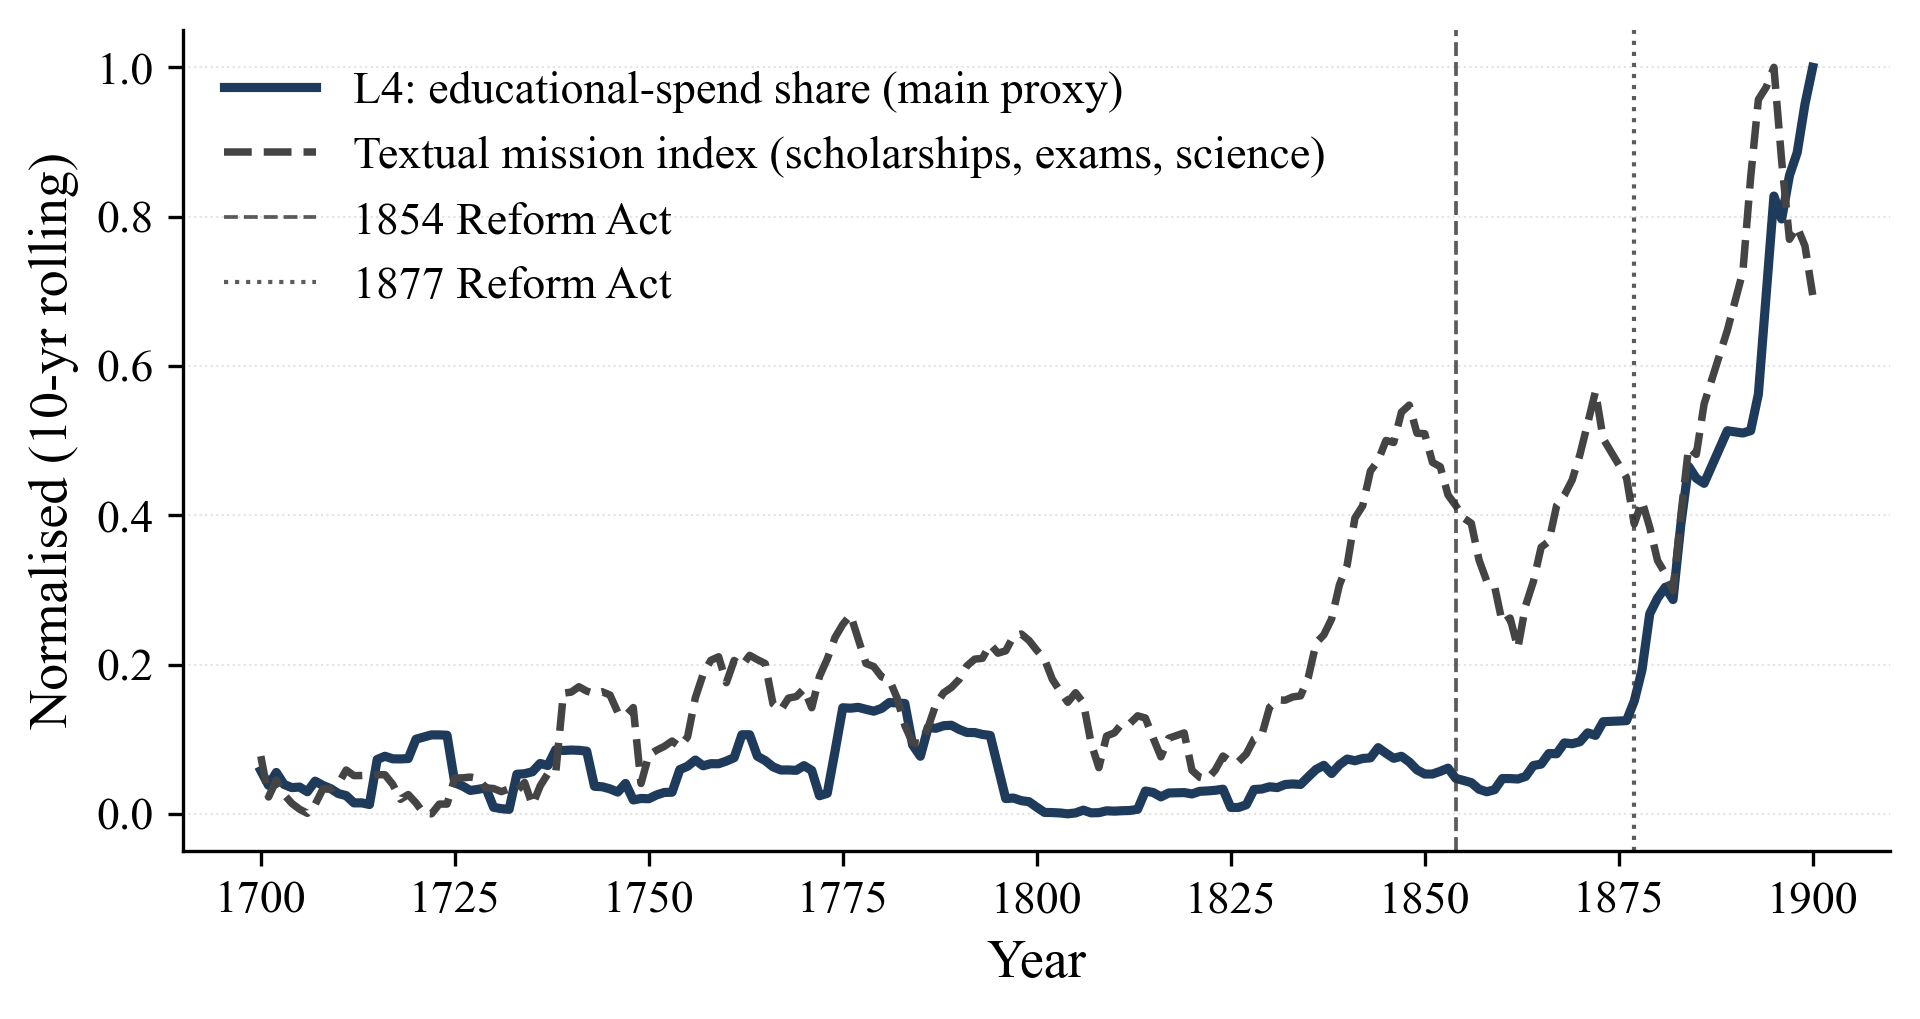
\includegraphics[width=0.66\textwidth]{figures/fig_l4_triangulation.png}
\caption{L4 validation. The educational-spend share (the main L4 proxy) and an independent
textual mission index (scholarships, prizes, examinations, teaching, scientific vocabulary) both
rescaled to $[0,1]$ on 10-year rolling means. The two move together (trend $r = 0.75$),
indicating that the mission proxy captures a real reallocation of purpose.}
\label{fig:l4tri}
\end{figure}

% ===========================================================================
\section{Empirical Strategy}
\label{sec:methods}
% ===========================================================================

We deploy complementary strategies, each addressing a distinct facet of the depth-asymmetry
claim.

\paragraph{Interrupted time series (ITS).} For each depth $y_t$ we estimate
\begin{equation}
\label{eq:its}
y_t = \beta_0 + \beta_1 t + \beta_2 D^{54}_t + \beta_3 (t-1854)D^{54}_t + \beta_4 D^{77}_t + \beta_5 (t-1877)D^{77}_t + \varepsilon_t,
\end{equation}
where $D^{54}_t, D^{77}_t$ indicate the post-1854 and post-1877 regimes. Coefficients $\beta_2,
\beta_4$ measure level shifts; $\beta_3, \beta_5$ measure trend breaks. We report HAC standard
errors (max lag 10) and normalise each level shift by the depth's own pre-reform mean to compare
across scales.

\paragraph{Structural-break detection.} To confirm reform years are genuine break-points, we
apply binary-segmentation change-point detection (RBF kernel, minimum segment 8 years) to each
series and report the largest break relative to its pre-break segment mean.

\paragraph{Discontinuity sharpness.} Two measures test whether reform shifts are discontinuous.
The signal-to-noise ratio $\text{SNR}_k = |\bar{y}^{\text{post}}_k - \bar{y}^{\text{pre}}_k| /
\overline{\sigma}^{\text{pre}}_{k,10\text{yr}}$ compares the break to baseline volatility. The
sharpness index $\text{Sharpness}_k = (\bar{y}^{[1854,1859)}_k - \bar{y}^{\text{pre}}_k)/
(\bar{y}^{\text{post}}_k - \bar{y}^{\text{pre}}_k)$ measures the share of total post-reform gain
realised in the first five years; under a uniform linear trend it equals $5/n_{\text{post}}
\approx 0.135$.

\paragraph{Regime conditioning.} To test whether depths respond differently under disruption
than under calm (H1), we classify each year as ``disruption'' ($\pm 8$ years around a reform) or
``calm,'' and compare each depth's year-on-year movement, normalised by its own scale, across
regimes.

\paragraph{Persistence decomposition.} To test durability (H2), we decompose each depth's
post-reform change into the gain realised in the decade after 1877 and the fraction \emph{held}
through 1891--1900, classifying each as durable, transitory, or no-gain.

\paragraph{Lock-in counterfactual.} To test the efficiency trap (H3), we construct a
counterfactual transformation index for an organisation that changed only at the operational
depths (L1/L2), holding the higher depths at baseline, and compare it to the actual trajectory.

\paragraph{Causal robustness.} Because the leapfrogging interpretation rests on the reforms
\emph{causing} the higher-order response, we corroborate the ITS with a battery of identification
checks applied to the combined higher-order axis, the \emph{modern-function share}
$\text{MFS}_t = (\text{educational} + \text{salary/stipend})_t / \text{total expenditure}_t$,
i.e.\ L3 and L4 jointly. These comprise sharp regression-discontinuity (RDD) estimates at each
reform cutoff across bandwidths; local-projection impulse responses tracing the dynamic effect
over subsequent horizons; Granger tests of whether resource slack ($\lambda$) leads MFS; and
placebo-in-time cutoffs. We read these jointly: identification rests on the convergence of
complementary tests, not on any single one.

% ===========================================================================
\section{Results}
\label{sec:results}
% ===========================================================================

The results build a single argument in five steps. We first show that the four depths followed
distinct trajectories; that the higher depths responded disproportionately, and discontinuously,
to the reform shocks; that this response was specific to disruption rather than to the passage of
time; that only the mission depth left a durable mark; and finally, by counterfactual, that an
organisation confined to the operational depths would have stagnated. Each step is carried by a
figure or table and the numbers behind it.

\subsection{Four depths over two centuries}

Figure~\ref{fig:dim} plots the four depths over 1700--1900. The series have clearly distinct
profiles: L1 (efficiency) rises through the 18th century and stabilises near 0.8; L2 (process)
is high throughout with mild drift; L3 (capability) is the most volatile; L4 (mission) is small
throughout the pre-reform period and rises sharply only in the late 19th century. Era-level
means (Table~\ref{tab:era}) make the asymmetry concrete: from the early- to the late-industrial
era, L4 jumps roughly ninefold (0.016 $\to$ 0.138) while L1 and L2 are essentially flat and L3
actually declines.

\begin{figure}[t]
\centering
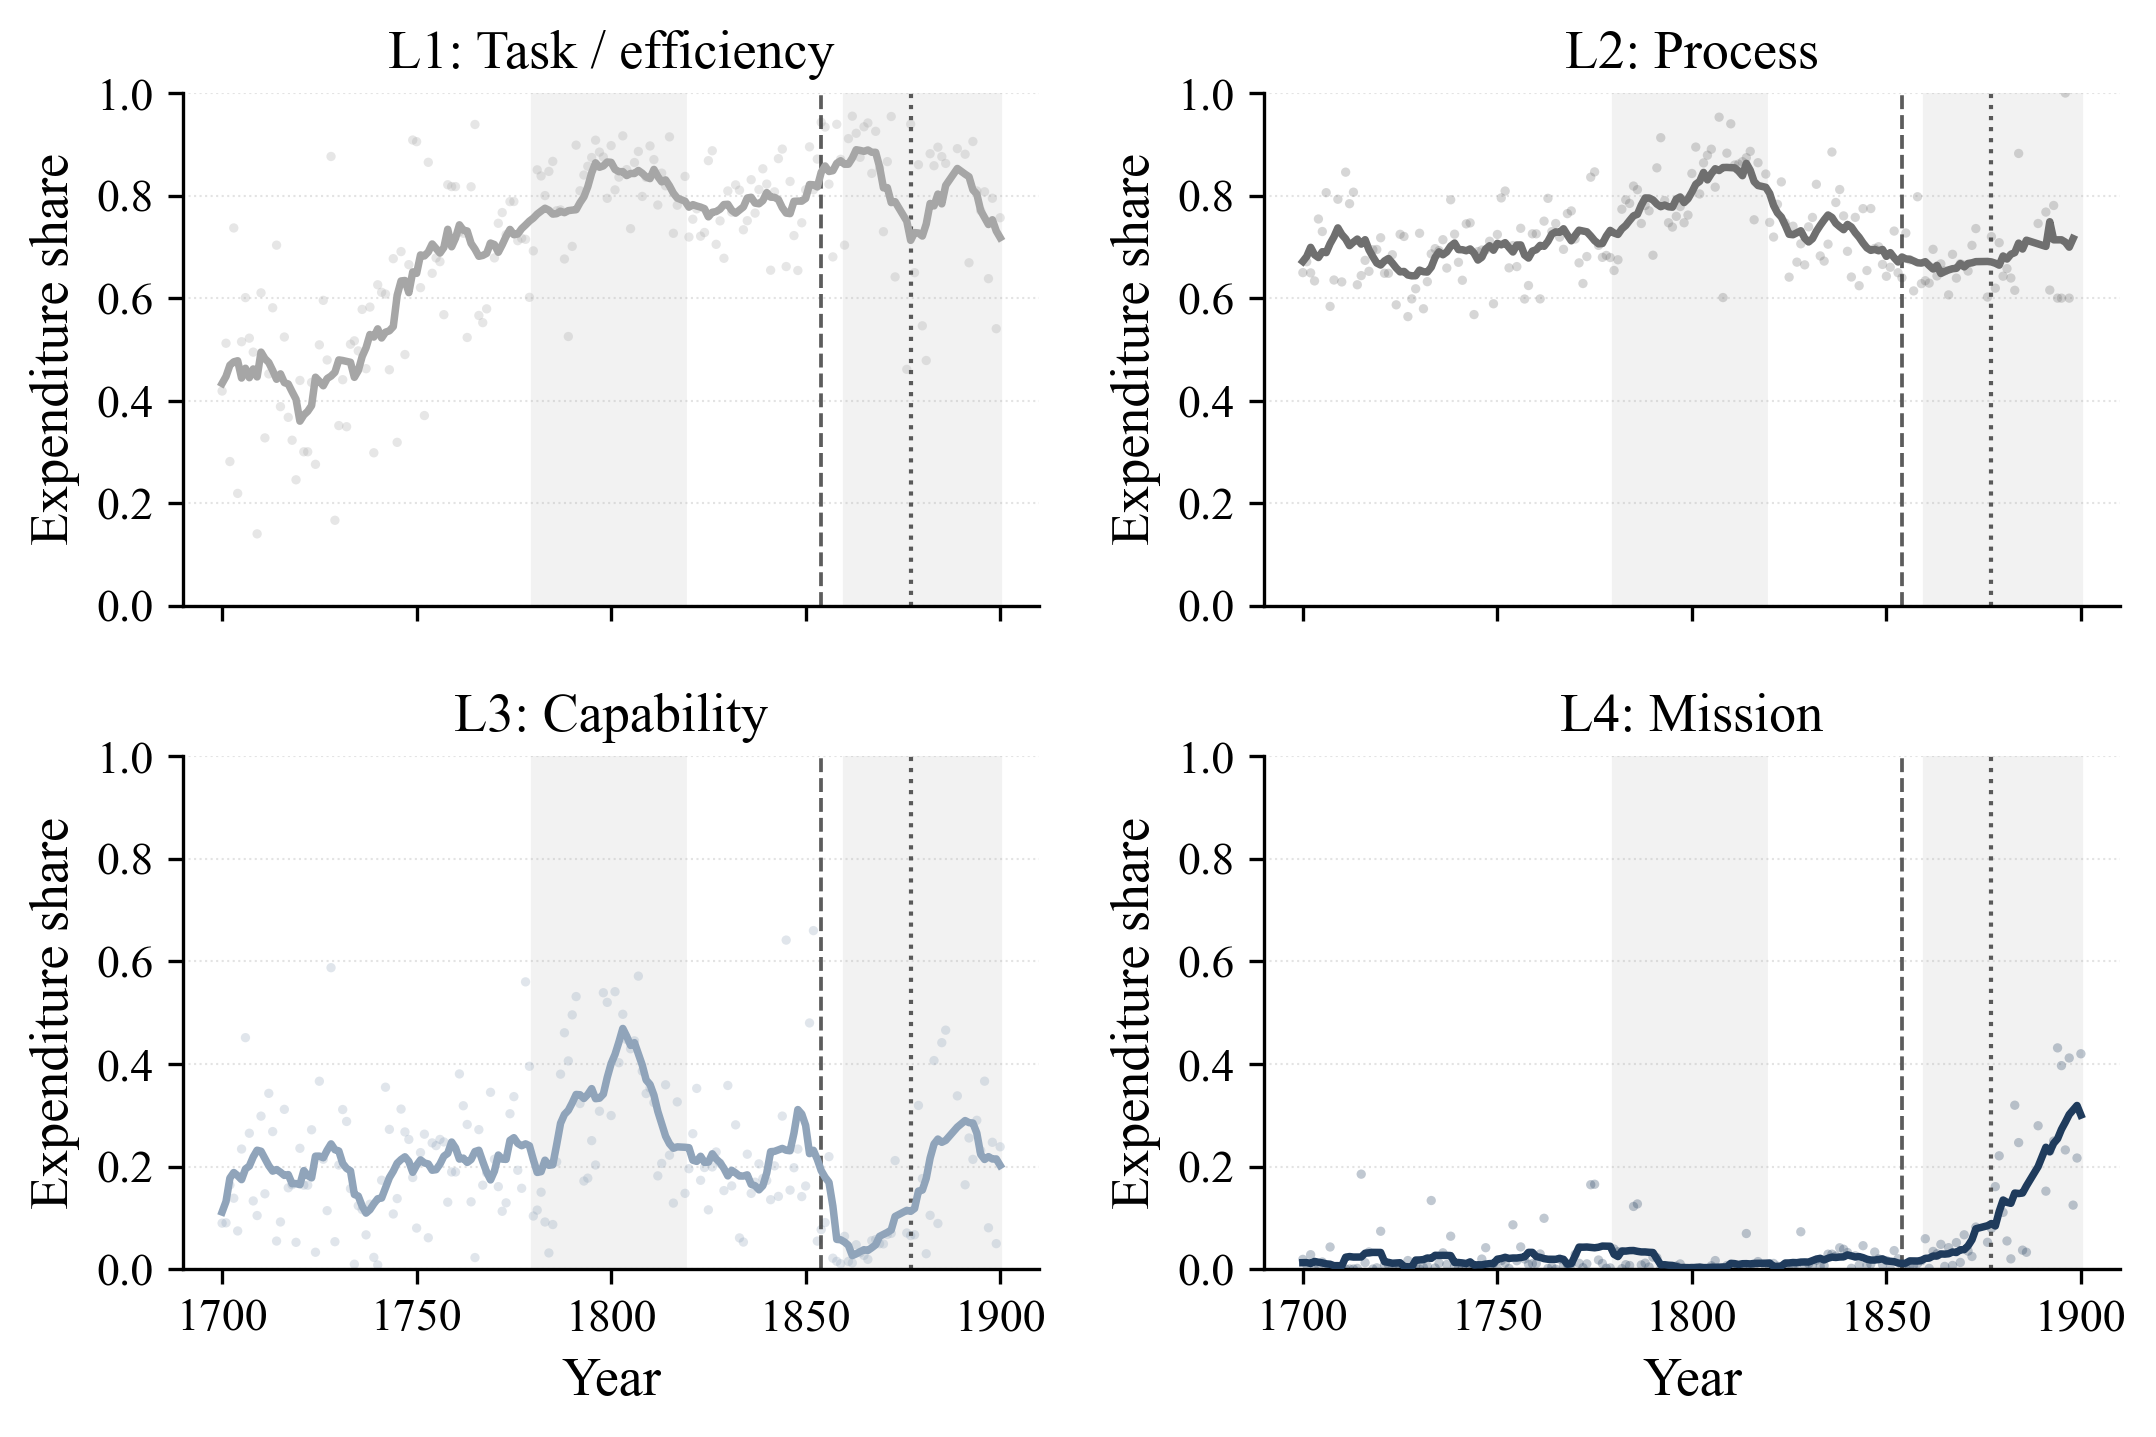
\includegraphics[width=0.80\textwidth]{figures/fig_dimensions.png}
\caption{The four transformation depths of Oxford University, 1700--1900. Points are annual
values; lines are 10-year centred rolling means. Vertical lines mark the 1854 and 1877 Reform
Acts; shaded bands denote era classification.}
\label{fig:dim}
\end{figure}

\begin{table}[t]
\centering
\caption{Era-level mean transformation depths}
\label{tab:era}
\small
\begin{tabular}{lcccccc}
\toprule
Era & Years & $n$ & L1 & L2 & L3 & L4 \\
\midrule
Pre-industrial   & 1700--1779 & 80 & 0.564 & 0.695 & 0.202 & 0.021 \\
Transition       & 1780--1819 & 39 & 0.820 & 0.809 & 0.312 & 0.015 \\
Early-industrial & 1820--1859 & 40 & 0.794 & 0.715 & 0.201 & 0.016 \\
Late-industrial  & 1860--1900 & 36 & 0.801 & 0.680 & 0.153 & 0.138 \\
\bottomrule
\end{tabular}
\end{table}

\subsection{Leapfrogging: disproportionate higher-depth response (H1)}

Figure~\ref{fig:norm} normalises each depth to its 1820--1853 pre-reform mean. If transformation
were uniform, the four trajectories would diverge similarly; they do not. L4 rises multiple-fold
above baseline after 1854, while L1 and L2 stay near 1.0 throughout. This upward divergence of
the strategic axis against a flat operational axis is the leapfrogging signature.

\begin{figure}[t]
\centering
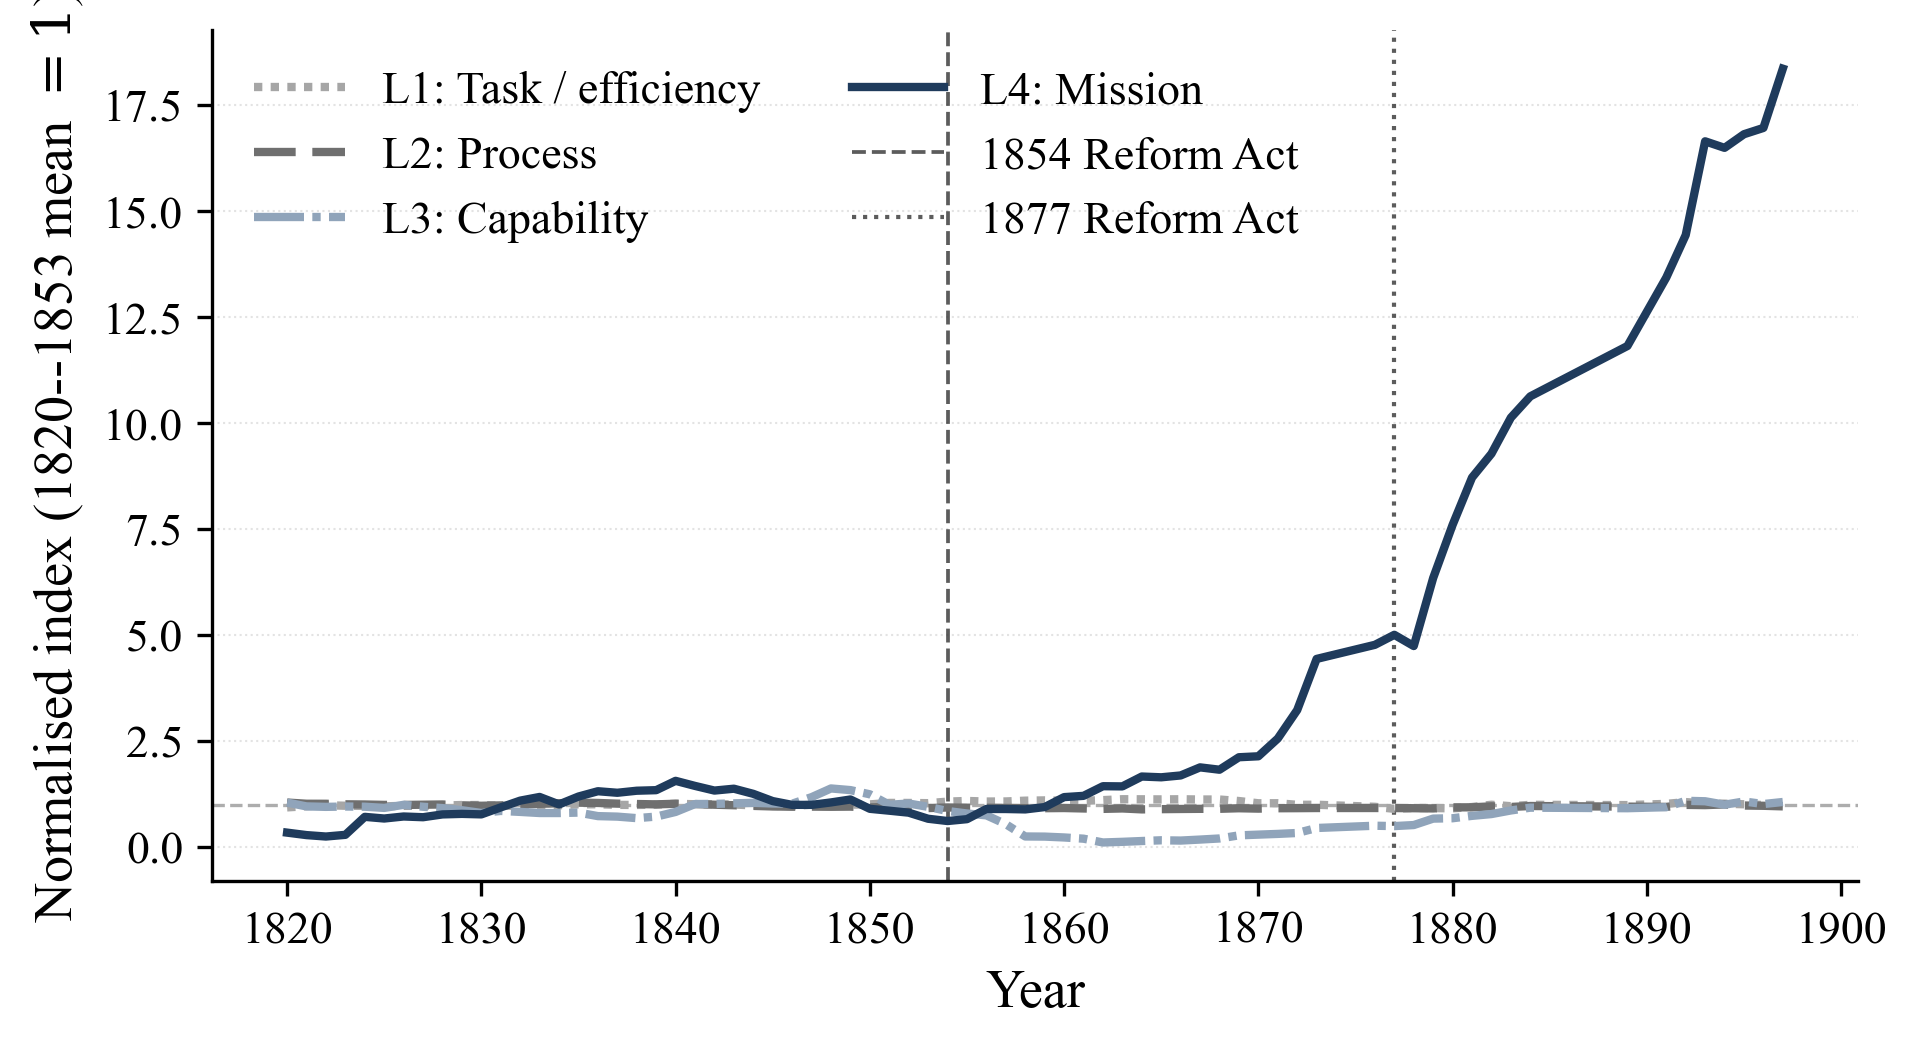
\includegraphics[width=0.72\textwidth]{figures/fig_normalised.png}
\caption{Normalised growth trajectories, 1820--1900, each rescaled to its 1820--1853 pre-reform
mean. Leapfrogging is visible as the disproportionate divergence of L4 above the L1/L2 baseline.}
\label{fig:norm}
\end{figure}

The ITS estimates (Table~\ref{tab:its}, Figure~\ref{fig:its}) sharpen the picture. At 1854, L3
and L4 show large \emph{negative} shifts (an initial disruption) while L1 and L2 barely move; at
1877, L3 and L4 show large \emph{positive} shifts (acceleration), again with L1 and L2 flat. The
L4 normalised level shift at 1877 is $2.41\times$ its pre-reform mean, roughly 60 times the L1
effect ($0.04\times$) and 93 times the L2 effect ($0.03\times$).

\begin{table}[t]
\centering
\caption{Interrupted time series: level-shift coefficients normalised by pre-reform mean}
\label{tab:its}
\small
\begin{tabular}{llrrrl}
\toprule
Depth & Reform & Coef. & SE & $p$ & Norm. effect \\
\midrule
L1 (Efficiency) & 1854 & $+0.018$ & 0.058 & 0.764 & $+0.026$ \\
L1 (Efficiency) & 1877 & $+0.027$ & 0.071 & 0.699 & $+0.040$ \\
L2 (Process)    & 1854 & $-0.107$ & 0.033 & 0.001 & $-0.146$\textsuperscript{***} \\
L2 (Process)    & 1877 & $+0.019$ & 0.019 & 0.309 & $+0.026$ \\
L3 (Capability) & 1854 & $-0.235$ & 0.047 & 0.000 & $-1.001$\textsuperscript{***} \\
L3 (Capability) & 1877 & $+0.070$ & 0.040 & 0.082 & $+0.299$\textsuperscript{*} \\
L4 (Mission)    & 1854 & $-0.013$ & 0.005 & 0.013 & $-0.679$\textsuperscript{**} \\
L4 (Mission)    & 1877 & $+0.045$ & 0.014 & 0.002 & $+\mathbf{2.408}$\textsuperscript{***} \\
\bottomrule
\end{tabular}

\medskip
\footnotesize\textit{Notes:} HAC SE (max lag 10). \textsuperscript{*}$p<0.10$,
\textsuperscript{**}$p<0.05$, \textsuperscript{***}$p<0.01$. Normalised effect $=$ coef.\ /
pre-reform mean.
\end{table}

\begin{figure}[t]
\centering
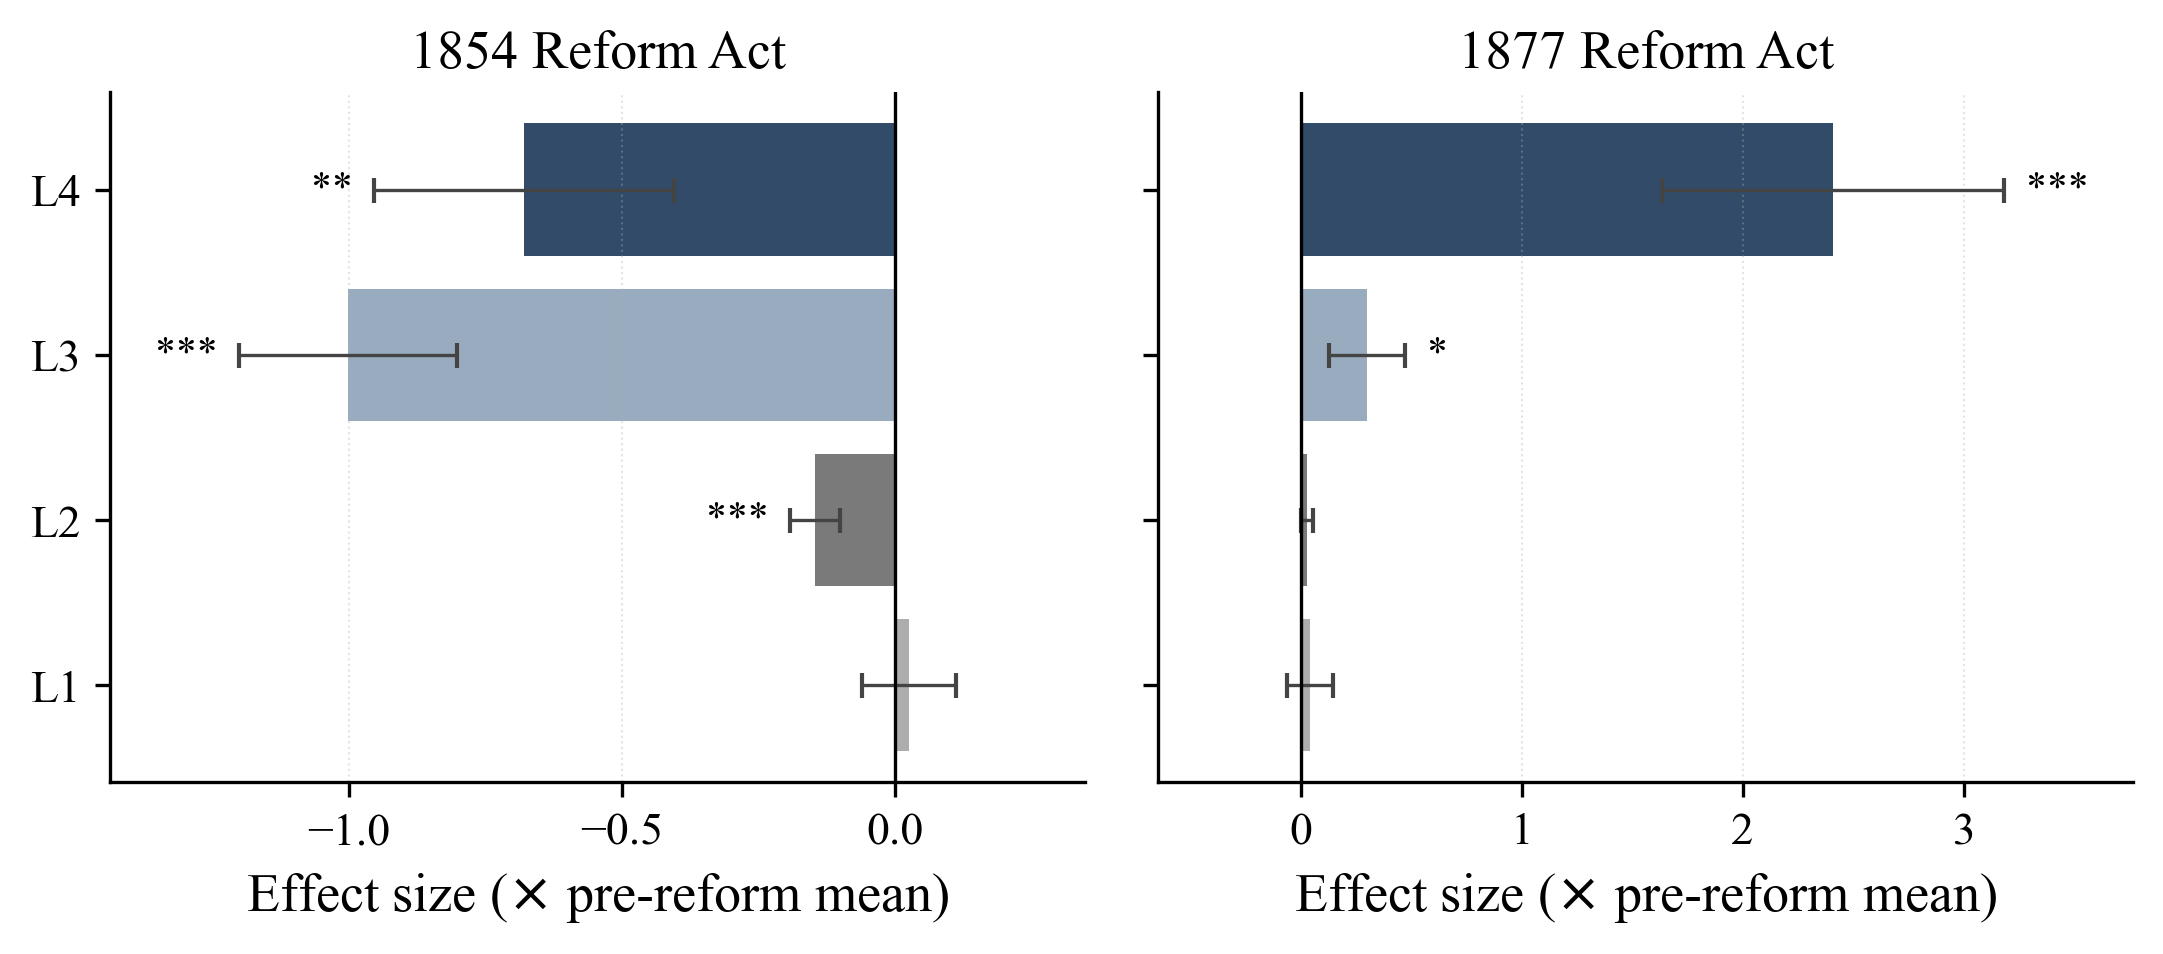
\includegraphics[width=0.82\textwidth]{figures/fig_its_effects.png}
\caption{Normalised ITS level-shift effects by depth at each Reform Act (coefficient divided by
the depth's pre-reform mean). Error bars are HAC standard errors, similarly normalised; stars
denote significance.}
\label{fig:its}
\end{figure}

The structural-break magnitudes (Table~\ref{tab:breaks}, Figure~\ref{fig:breaks}) are the single
most striking piece of evidence. L4's largest break is $3.63\times$ its pre-break mean, an
order of magnitude larger than L2's ($0.06\times$) and roughly six times L1's ($0.64\times$),
even after accounting for scale.

\begin{table}[t]
\centering
\caption{Largest structural break by depth (binary segmentation)}
\label{tab:breaks}
\small
\begin{tabular}{llrrr}
\toprule
Depth & Break year & Pre-break mean & Post-break mean & Rel.\ magnitude \\
\midrule
L1 (Efficiency) & 1750 & 0.480 & 0.785 & $0.64\times$ \\
L2 (Process)    & 1780 & 0.695 & 0.739 & $0.06\times$ \\
L3 (Capability) & 1851 & 0.231 & 0.142 & $0.39\times$ \\
L4 (Mission)    & 1836 & 0.018 & 0.084 & $\mathbf{3.63\times}$ \\
\bottomrule
\end{tabular}

\medskip
\footnotesize\textit{Notes:} RBF kernel, min.\ segment 8 years. Rel.\ magnitude $=
|\bar{y}^{\text{post}}-\bar{y}^{\text{pre}}|/\bar{y}^{\text{pre}}$.
\end{table}

\begin{figure}[t]
\centering
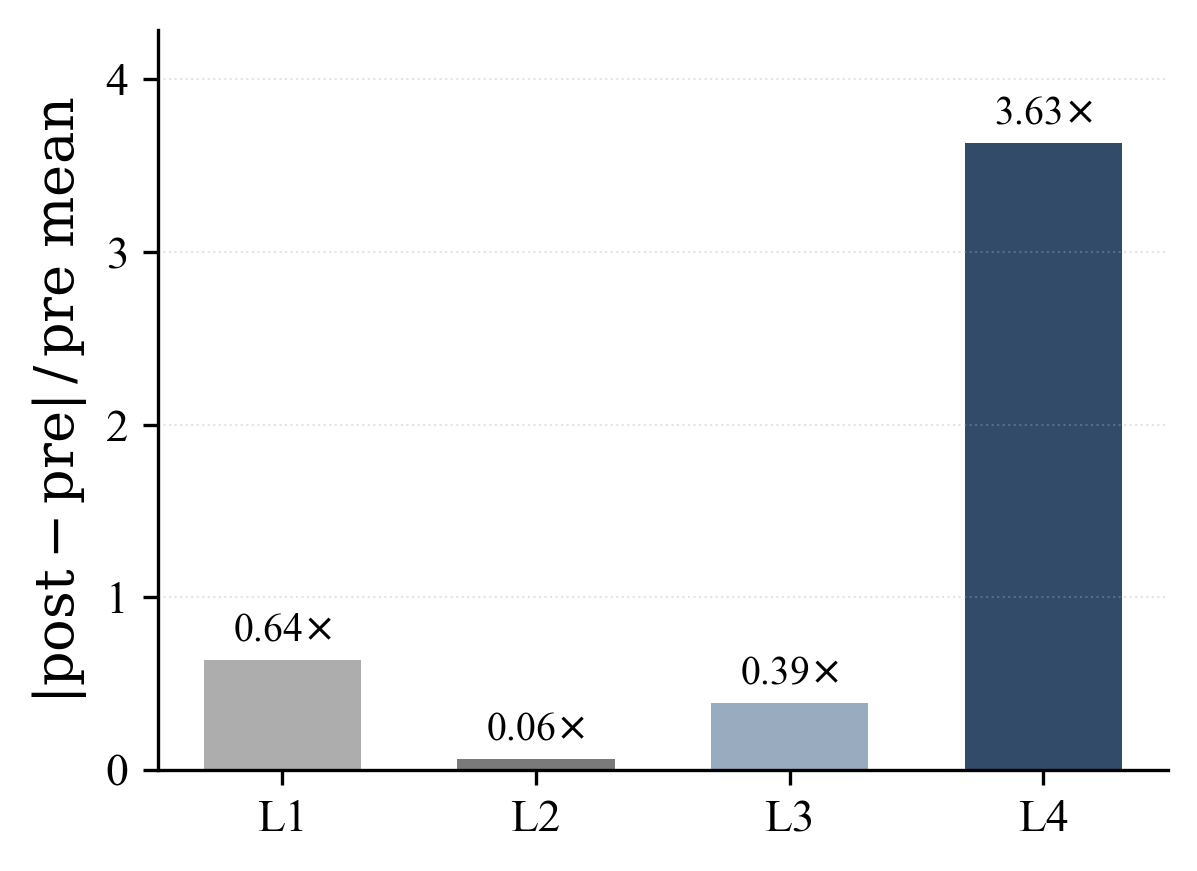
\includegraphics[width=0.46\textwidth]{figures/fig_breaks.png}
\caption{Relative break magnitude by depth: the largest detected structural break divided by its
pre-break segment mean.}
\label{fig:breaks}
\end{figure}

\subsection{Reform Acts as strategic discontinuities}

Leapfrogging presupposes that the reforms induced discontinuous, not gradual, change.
Figure~\ref{fig:disc} confirms this. Signal-to-noise ratios for the 1854 break are at or above
typical year-to-year volatility for L1 (1.50), L2 (0.99), and L3 (1.53); L4's lower SNR (0.37)
reflects its much smaller absolute scale, not weak discontinuity (its \emph{relative} break is
the largest in the dataset). The sharpness index shows that for L1 (1.35), L2 (0.78), and L3
(1.32) the bulk of post-1854 change occurred in the first five years, six to ten times the
linear-trend expectation of $0.135$, indicating concentrated, punctuated reorganisation.

\begin{figure}[t]
\centering
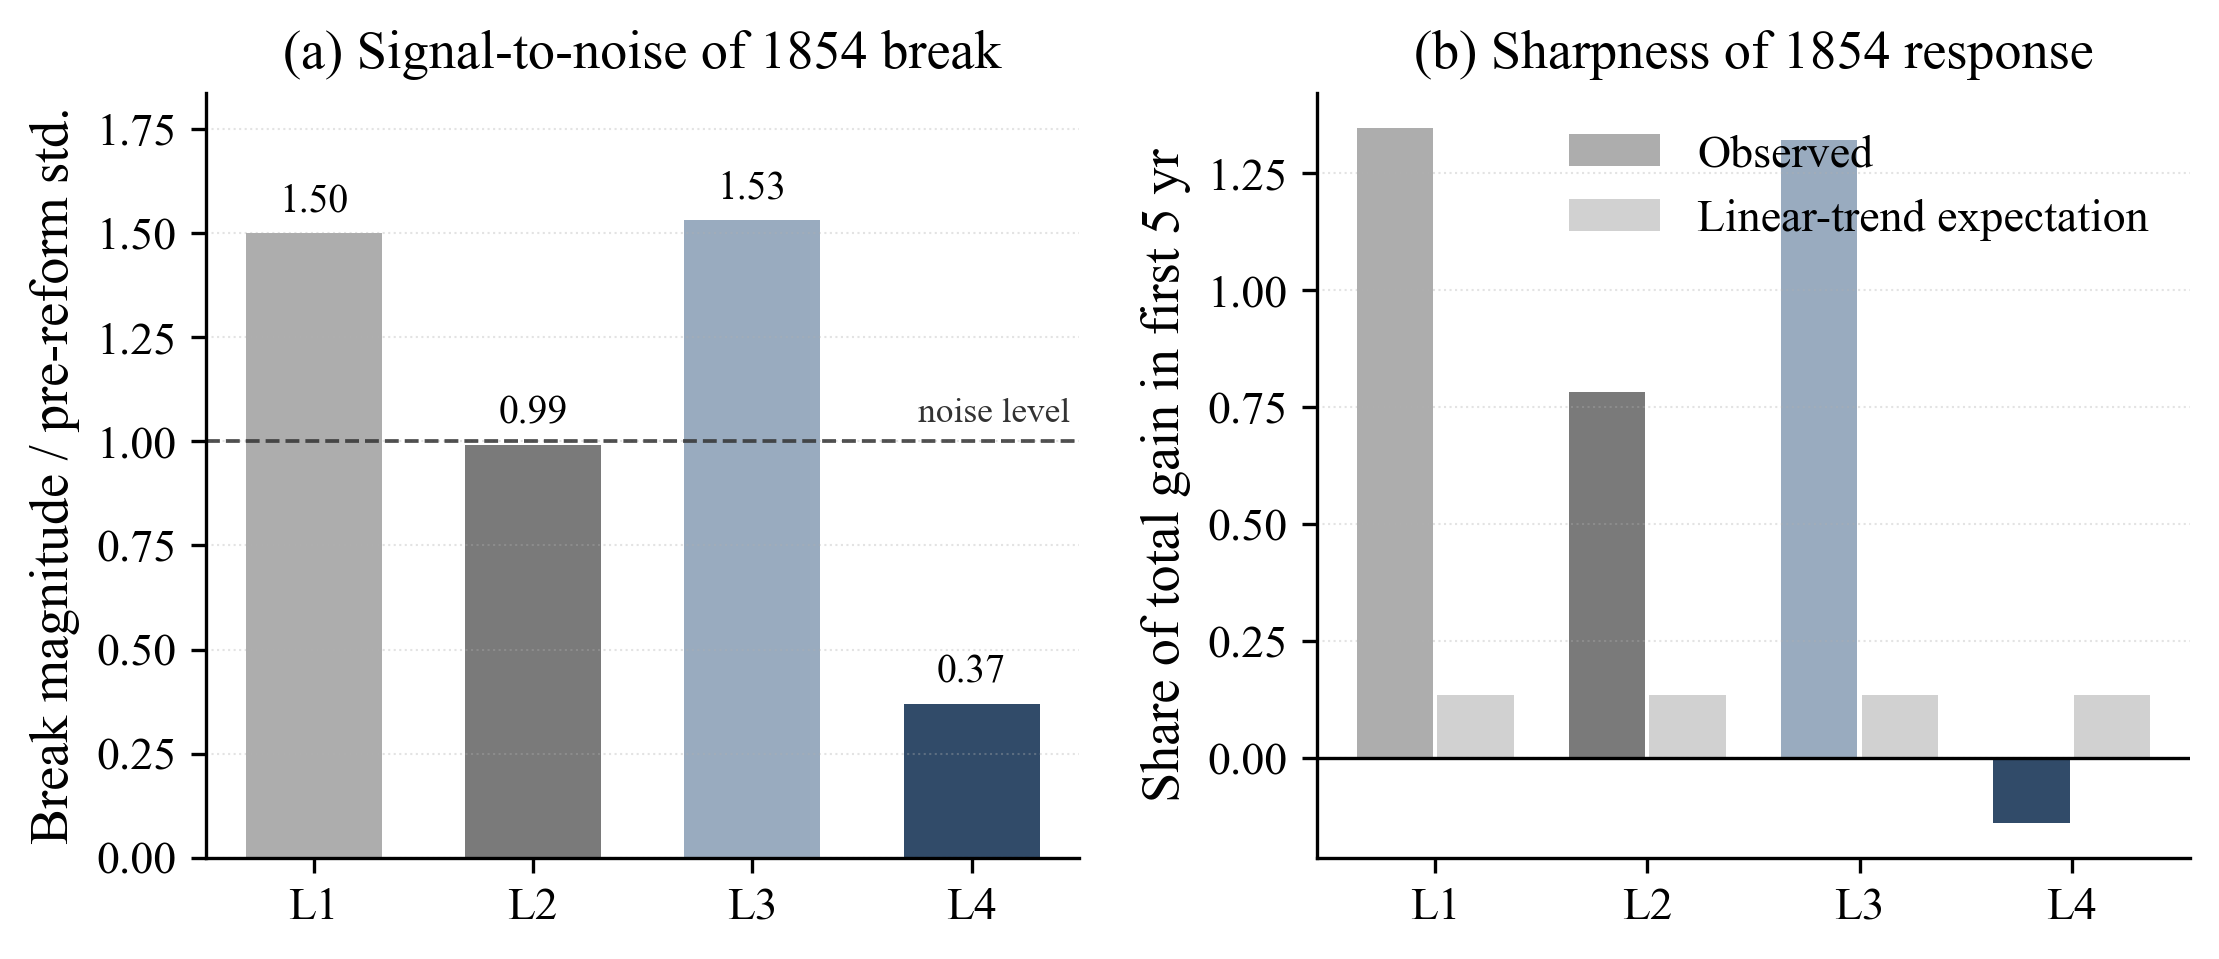
\includegraphics[width=0.85\textwidth]{figures/fig_discontinuity.png}
\caption{Reforms as discontinuities. (a) Signal-to-noise ratio of the 1854 break by depth
(break magnitude / pre-reform rolling std.); the dashed line marks the noise level. (b) Sharpness:
observed share of total post-1854 gain realised in the first five years versus the share expected
under a uniform linear trend.}
\label{fig:disc}
\end{figure}

\subsection{Robustness: the reforms as causal discontinuities}

The depth-asymmetry results rely on the reforms being causal, not coincidental. We corroborate
this on the combined higher-order axis (MFS $=$ L3 $+$ L4). Figure~\ref{fig:causal}(a) plots MFS
against the no-reform ITS counterfactual: after 1854 the higher-order axis departs from the
trajectory it would have followed absent the reforms. Figure~\ref{fig:causal}(b) reports
regression-discontinuity estimates at each cutoff. The 1854 reform produces a robust negative
level discontinuity in MFS ($\tau \approx -0.25$ at a 15-year bandwidth, $p = 0.02$; stable
across bandwidths), matching the initial-disruption sign of the 1854 ITS shifts; the 1877 cutoff
shows no \emph{level} discontinuity ($\tau \approx 0.03$--$0.06$, n.s.), consistent with 1877
acting through a trend acceleration rather than a one-off jump. Local projections show an
immediate higher-order response (horizon $h{=}0$: $0.17$, $p = 0.01$; $h{=}1$: $0.15$,
$p = 0.01$) that fades within two years, the same transitory signature we see for capability
(L3). Granger tests do not find resource slack leading MFS ($p > 0.15$ at all lags), reinforcing
our treatment of slack as a suggestive enabler rather than a demonstrated driver. We note one
honest limitation: because the higher-order axis was already drifting during the early-industrial
transition, placebo-in-time cutoffs in the 1820s also register; this is why we lean on the
\emph{convergence} of ITS, RDD, break detection, and sharpness rather than any single test.

\begin{figure}[t]
\centering
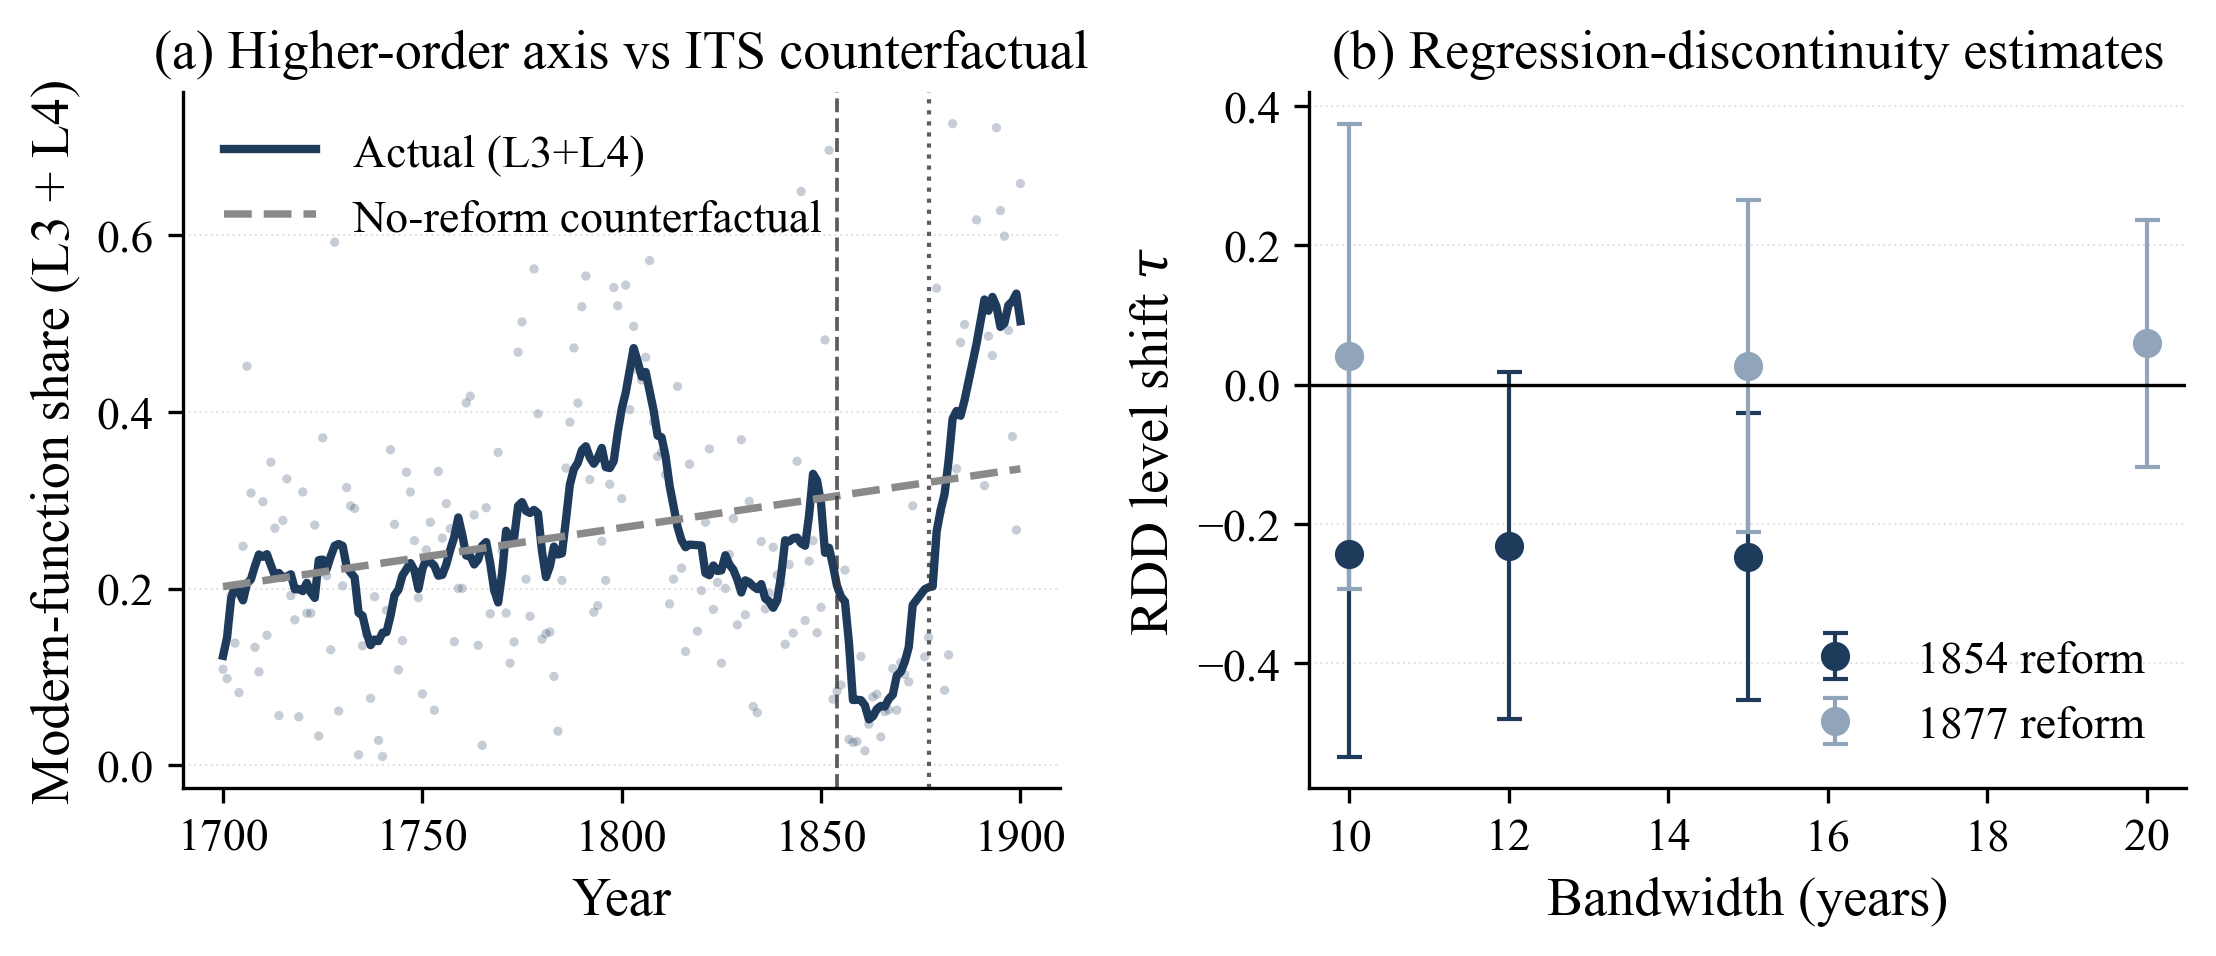
\includegraphics[width=0.85\textwidth]{figures/fig_causal_robustness.png}
\caption{Causal robustness on the higher-order axis (MFS $=$ L3 $+$ L4). (a) Actual
modern-function share versus the no-reform ITS counterfactual. (b) Regression-discontinuity
level-shift estimates $\tau$ at the 1854 and 1877 cutoffs across bandwidths, with 95\% confidence
intervals. The 1854 discontinuity is robustly negative; the 1877 cutoff shows no level jump.}
\label{fig:causal}
\end{figure}

\subsection{Which depths move under disruption versus calm? (H1)}

Figure~\ref{fig:cond} compares each depth's movement, normalised by its own scale, in calm years
versus disruption windows ($\pm 8$ years around a reform). The mission depth (L4) is the most
disruption-driven: its normalised movement is 2.59 in disruption versus 1.74 in calm, and its
movement is the most concentrated in shock years of any depth (concentration index 1.38). The
process depth (L2) is the least disruption-driven: its concentration index (0.94) is below
neutral, identifying it as steady \emph{background} infrastructure that improves regardless of
shocks. L1 and L3 are intermediate. This regime contrast is the clearest expression of the depth
asymmetry: \emph{the deeper the transformation, the more it is a response to disruption rather
than to ordinary time.}

\begin{figure}[t]
\centering
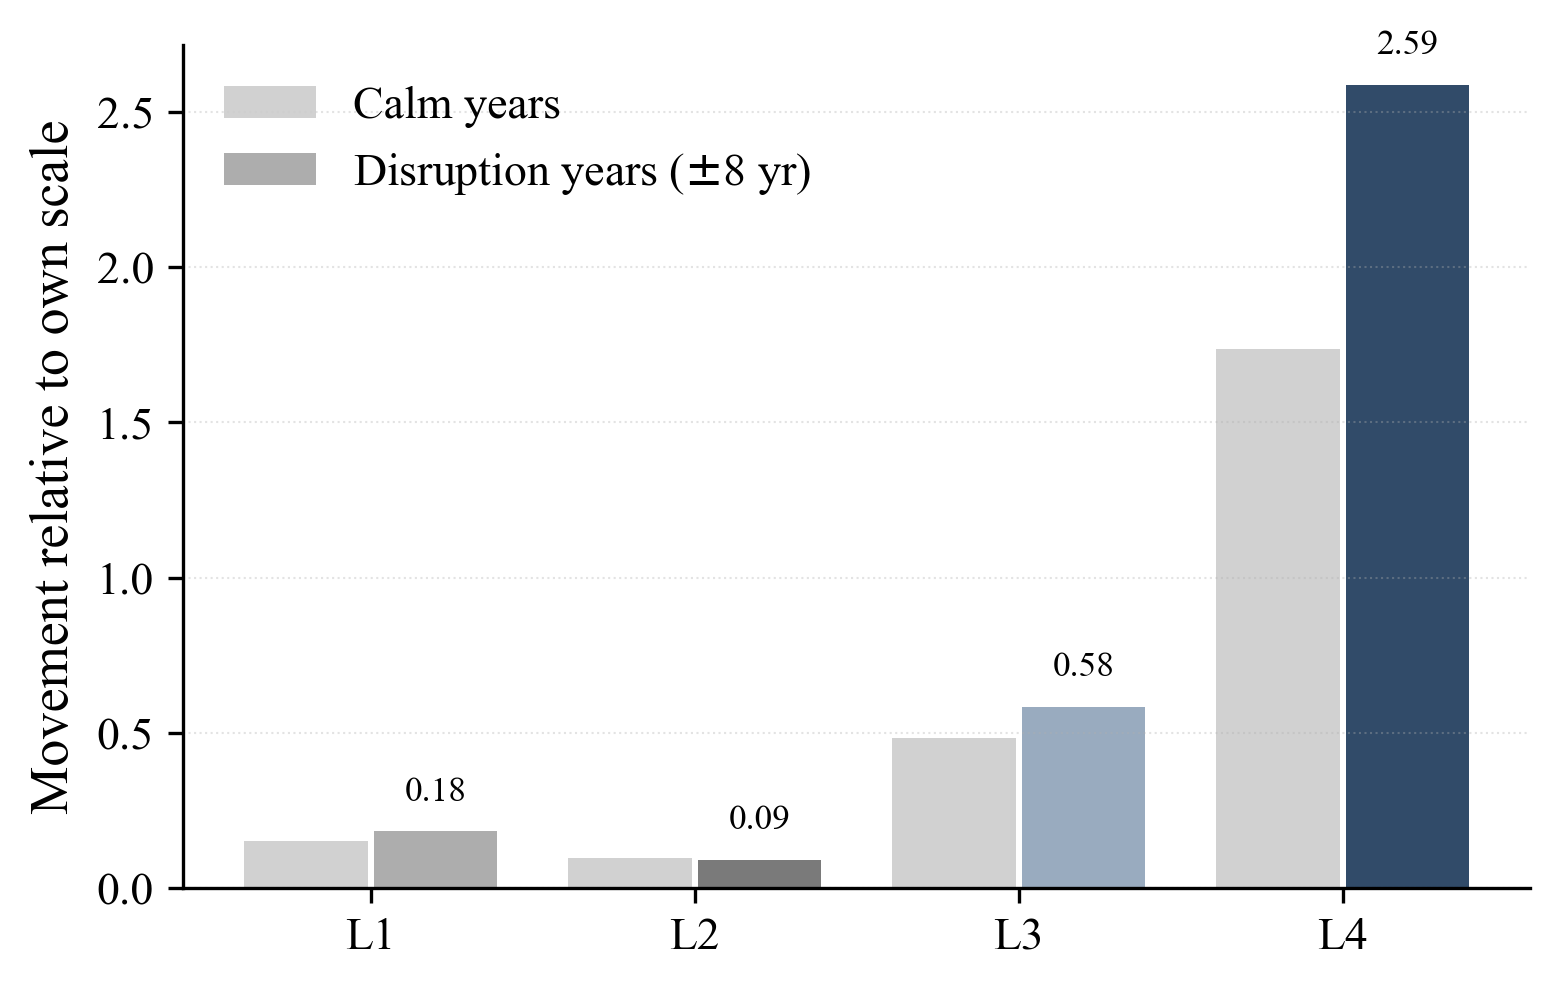
\includegraphics[width=0.56\textwidth]{figures/fig_conditioning.png}
\caption{Depth movement by environmental regime. Bars show each depth's movement relative to its
own scale, in calm years (grey) versus disruption windows ($\pm 8$ years around a reform,
coloured). L4 moves most under disruption; L2 is steady background.}
\label{fig:cond}
\end{figure}

\subsection{Only the mission depth endures (H2)}

A large response is not the same as a lasting one, and the two need not coincide.
Figure~\ref{fig:pers} decomposes durability. Only L4 shows a \emph{sustained} gain held through
1891--1900 ($+0.269$ retained); L3 capability is \emph{transitory} (it rises around reforms then
reverts); and L1 and L2 show \emph{no durable gain} at all. The durable transformation that
remains by the end of the period is, almost entirely, mission-level.

\begin{figure}[t]
\centering
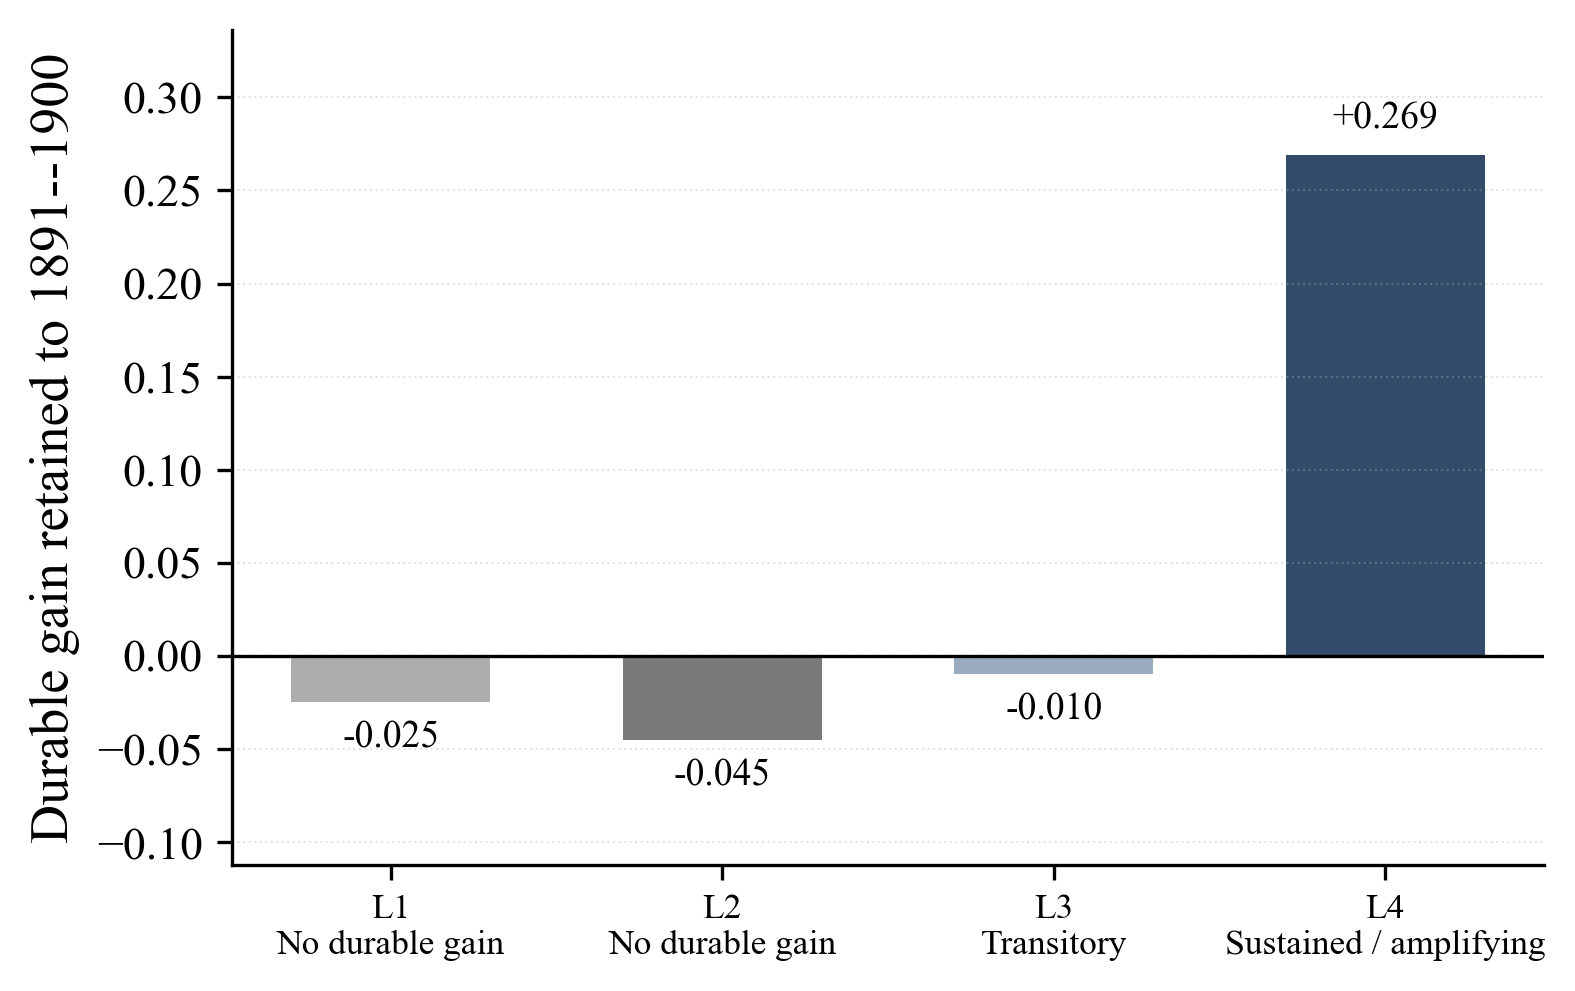
\includegraphics[width=0.55\textwidth]{figures/fig_persistence.png}
\caption{Durability of post-reform change by depth: the gain retained through 1891--1900. Only
the mission depth (L4) sustains its gain; capability (L3) is transitory; the operational depths
show no durable gain.}
\label{fig:pers}
\end{figure}

\subsection{The efficiency trap (H3)}

If only the higher depths endure, what would an organisation have gained by perfecting the lower
ones? Almost nothing, as it turns out. Figure~\ref{fig:trap} contrasts Oxford's actual
transformation trajectory with a counterfactual
organisation that changed only at the operational depths (L1/L2). The two are indistinguishable
before 1854; thereafter they diverge, and by the 1890s the higher-order contribution reaches
$+0.18$ to $+0.24$. Decomposed over 1820--1900, the operational-only path accounts for
essentially \emph{none} of the net durable change (and slightly regresses), while the higher
depths (L3/L4) account for the entire net durable transformation. An organisation optimising
only efficiency and process would have ended the period where it began.

\begin{figure}[t]
\centering
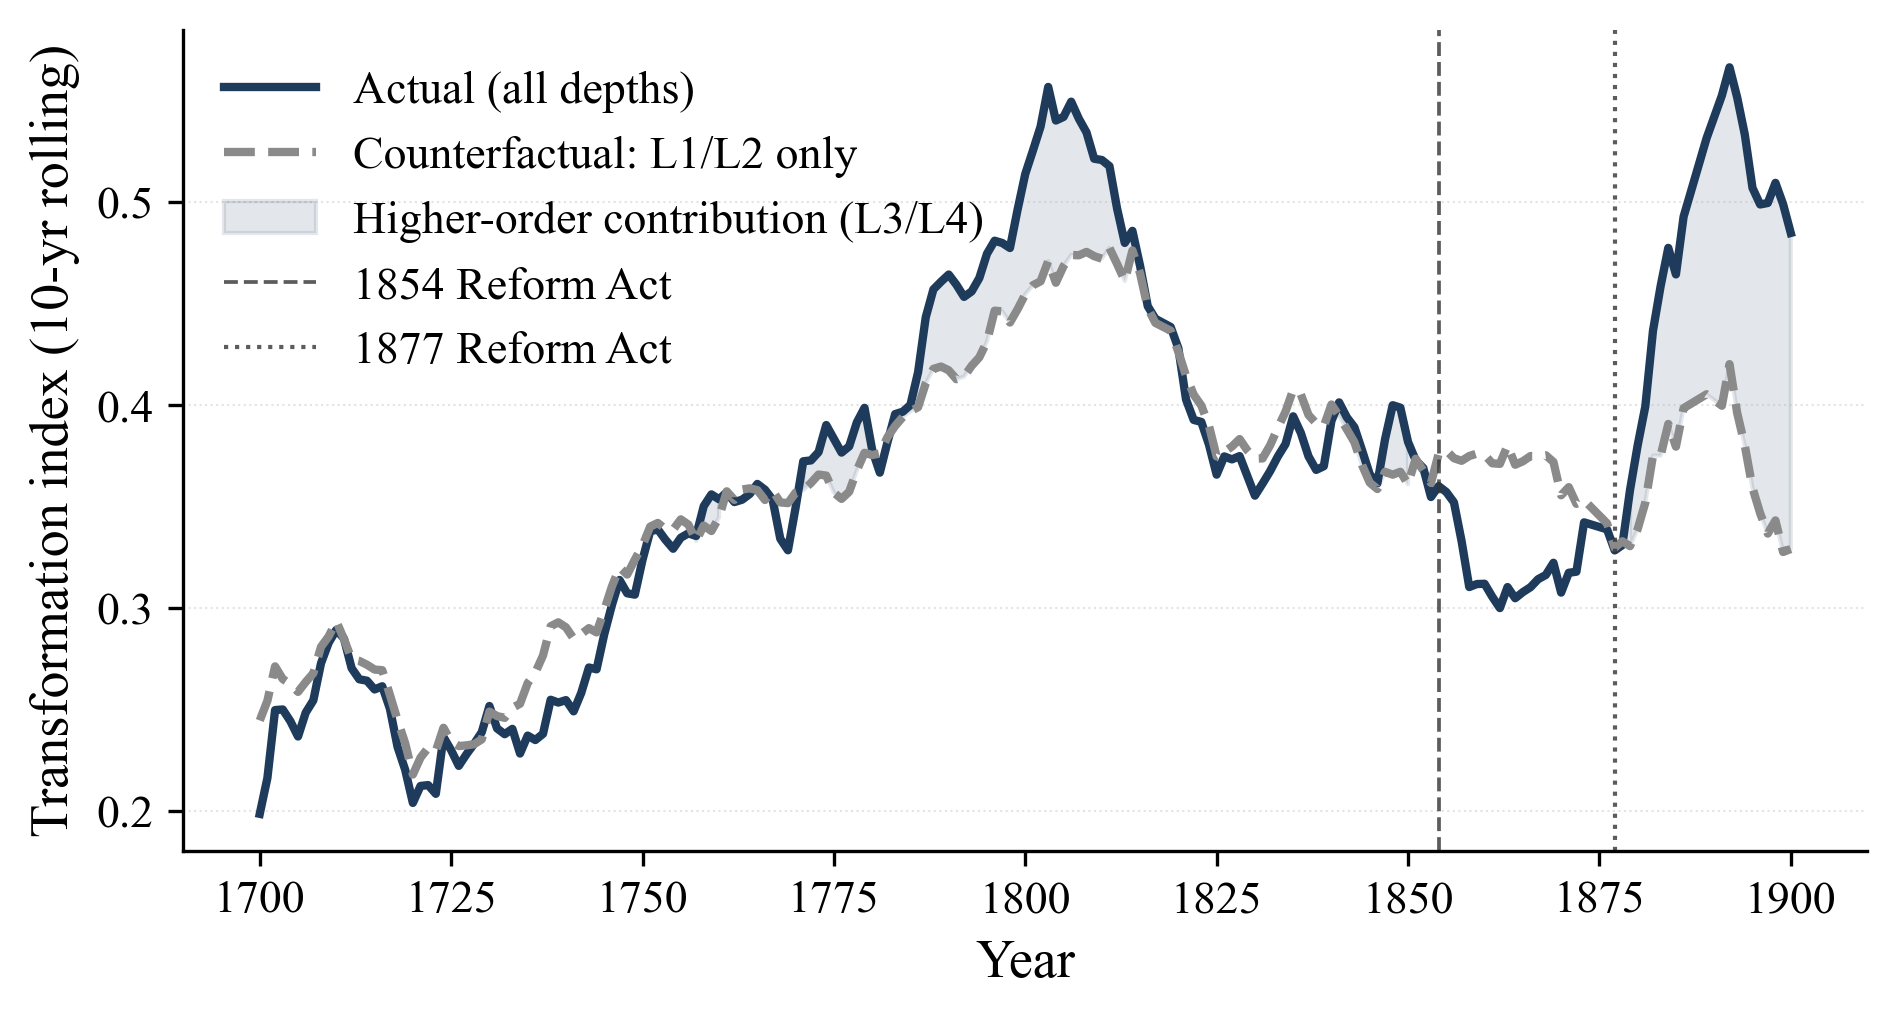
\includegraphics[width=0.66\textwidth]{figures/fig_efficiency_trap.png}
\caption{The efficiency trap. Actual transformation index (all depths) versus a counterfactual
that transforms only at the operational depths (L1/L2). The shaded area is the higher-order
(L3/L4) contribution, which accounts for the entire net durable change after 1854.}
\label{fig:trap}
\end{figure}

\subsection{Main versus exploratory findings}

Taken together, the five steps support the depth asymmetry along four robust lines: the higher
depths respond disproportionately to the reforms; that response is concentrated in disruption
rather than in calm; durable change is confined to the mission depth; and an efficiency-only path
stagnates. Each rests on several complementary tests rather than a single estimate. Two ideas
often associated with stage models, a strict L1$\rightarrow$L4 ordering and capability-before-mission
sequencing, are \emph{not} decisively supported, and we report them as exploratory nulls
(Appendix~\ref{app:inventory}); the resource-slack mechanism co-moves with the higher depths but
remains suggestive only. We carry only the robust claims into the discussion that follows.

% ===========================================================================
\section{Mechanism}
\label{sec:mechanism}
% ===========================================================================

We interpret the depth asymmetry as the product of three interacting forces. First, the Reform
Acts imposed \emph{exogenous strategic mandates} (expansion of teaching, abolition of
religious tests, restructuring of the fellowship system) that could not be met by marginal
efficiency improvement. In the terms of Section~\ref{sec:intro}, these mandates were the channel
through which industrial-era pressure, secular, scientific, and professional, reached a
corporation otherwise insulated from it. Second, the University's \emph{endowment-funded resource slack},
augmented by rising 19th-century land rents, provided the financial capacity to invest in
capability ahead of strategic clarity; consistent with this, slack co-moves with the higher
depths, although the lead-lag evidence is too weak to establish slack as a cause. Third, the
\emph{absence of competitive pressure} on Oxford's core mission meant operational optimisation
was not the binding constraint; external legitimacy was. Together these conditions produced a
textbook leapfrog: capability and mission moved first and discontinuously, while efficiency and
process modernised at their own slower internal pace.

% ===========================================================================
\section{Implications for AI Transformation}
\label{sec:ai}
% ===========================================================================

Oxford is not an AI case; what follows are lessons drawn by analogy from a completed
transformation, not claims about how organisations are responding to AI today. Read that way, the
depth asymmetry points to three things that any general-purpose-technology shock reshapes at once:
which inputs matter, which talent is required, and which business model wins.

\paragraph{Inputs: capital then, compute now.} A transformation has to be paid for, and at Oxford
the higher depths were gated less by intent than by resources. The instruments of the industrial
economy enter the ledgers on a datable timeline, government consols (1745), canal dividends
(1809), and the railway (1845), but they take decades to reshape the institution: the new
productive input is present long before its organisational payoff appears, exactly the lag that
the general-purpose-technology literature documents for steam, electricity, and computing
\citep{david1990dynamo, bresnahan1995gpt}. What let Oxford eventually convert that input into
mission change was a widening resource base, its revenue concentration first falls below an HHI of
$0.35$ in 1783, and the endowment and land-rent income that gave it slack; higher-order spending
moves with that income, even if the lead--lag is too weak to call slack a cause. The same logic
appears in the efficiency trap (Section~\ref{sec:results}): the organisation that cannot fund
L3/L4 stays stuck optimising L1/L2. The AI parallel is direct. Compute, and the capital to command
it, is the era's scarce productive input; resource-rich organisations can leapfrog, while
constrained ones are likelier to remain at the operational depths. This is the most tentative of
the three lessons, because our slack evidence is correlational, but it is also the most actionable:
budget slack for higher-order bets, because crisis urgency alone will not fund them.

\paragraph{Talent: a recomposition of who is paid.} The clearest signal in the archive is a change
in \emph{whom} the institution pays and for what. Payments to individuals fall from 16.3\% of
entries in the early 1700s to 4.7\% by 1900, while payments to institutions and salaried offices
rise from 1.7\% to 38.4\%, as casual and artisan labour gives way to professors, examiners, and a
permanent administration. This is the L3 capability dimension made concrete, and it is precisely
the skill-biased reorganisation that complementary-investment accounts associate with a major new
technology \citep{autor2003skill, bresnahan2002it}: the shock raises the return to skills that
complement the new input and lowers it for routine tasks. The lesson is that a technological shift
changes \emph{what talent an organisation needs}, and that this reallocation is part of the shock
response, not a consequence to be managed once the technology is in place.

\paragraph{Does a shock destroy work, or reallocate it?} A natural objection is that a
technological shock eliminates work rather than reshuffling it. Observed end to end, Oxford points
to reallocation. Real activity grew roughly $8.9\times$ over the period, and the labour the
institution paid for was recomposed rather than removed. New categories of paid work appear on a
datable timeline, with competitive examinations from 1737, scientific infrastructure from the
1750s, salaried lecturing and teaching from the 1770s, and a permanent salaried administration
later. Older
trades, meanwhile, persisted for generations rather than vanishing at once: the college's
glaziers, smiths, masons, and carpenters recur in the accounts across spans of 160 to 175 years,
overlapping the industrial suppliers that gradually displaced them. From primary records, this is
the pattern to which the historical-precedent argument in the contemporary debate over AI and jobs
appeals: paid work shifts and diversifies rather than simply disappearing.

Two caveats keep the lesson honest. First, the reallocation was slow, on the order of decades to a
century, and externally triggered rather than automatic; it produced losers as well as winners, as
craft, domestic, and clerical roles declined as durable shares of paid activity. Second, and more
telling for our argument, the labour build-up was not where durable value settled. Salaried
capability (L3) rose around the reforms and then receded, its share moving from 0.31 to 0.15,
while the lasting gain accrued to mission (L4). The organisational lesson is therefore sharper than
``reskill into the new roles'': retooling talent is necessary, but the durable advantage of a
transformation lies in redefining what the organisation does, not in the labour it reallocates. We
read the ledgers as evidence on the composition and organisation of paid work, not on employment
levels or wages, which the accounts do not record.

\paragraph{Business model: redefining what the organisation is.} Oxford's durable change was not
cheaper administration but a change in what the institution did and charged for. Teaching,
examination, and degree-granting moved to the centre, visible in new revenue logics such as
composition fees (first recorded in 1861) and in the educational mission's rise to the single
depth that durably grows (L4, retained at $+0.269$ to 1900). Lower-order modernisation accompanies
this, including the shift from Latin to English bookkeeping, but it is the redefinition of mission,
not the housekeeping, that endures. This is the sharpest lesson, because it rests on the paper's
strongest result: process improvement does not survive a genuine shock, durable advantage is
located at the business-model level, and under pressure the lower stages can be skipped.

In sum, four practical lessons follow. Treat automation and personalisation (L1/L2) as the
necessary baseline rather than the goal; locate durable advantage in mission and business-model
change (L4); budget explicit slack so higher-order bets can be funded; and reallocate talent, not
only tools, rather than managing transformation as a fixed maturity ladder that disruption will
not respect.



% ===========================================================================
\section{Boundary Conditions and What We Do Not Claim}
\label{sec:boundary}
% ===========================================================================

We are explicit about scope. The \emph{pace} of Oxford's transformation (200 years) is
pre-industrial and does not generalise to contemporary technology cycles; we claim the mechanism,
not the timescale. The \emph{institutional form} (an endowed, non-competitive Oxbridge
institution) is unusual; the closest contemporary analogue is a well-capitalised organisation
with substantial retained earnings, not the typical firm. The measures are ledger-based proxies:
L1 depends on a category boundary (which we fix and test), L2 is limited by payment-period
reliability, L3 is narrower than the full operating-model concept, and L4 is validated by textual
triangulation but cannot prove intentional strategy. We do \emph{not} find robust evidence for a
strict L1$\rightarrow$L4 ordering, nor decisive evidence that capability precedes mission once
series are detrended; we report these as disciplined nulls. We do \emph{not} establish resource
slack as a causal enabler, only as a co-moving, plausible precondition. And we do \emph{not}
test AI transformation: the analogy is a hypothesis for contemporary settings, not a result.

Another central boundary condition is that Oxford and AI differ in shock transmission. The Oxford case captures an institutionally mediated pathway of transformation, whereas AI adoption may begin as a bottom-up, tool-driven, and locally experimental process. This difference limits any direct analogy. At the same time, it sharpens the managerial implication: decentralized adoption may generate many L1/L2 improvements without producing durable transformation unless organizations develop mechanisms to aggregate local experiments into L3 operating-model reconfiguration and L4 mission/value redefinition.
% ===========================================================================
\section{Conclusion}
\label{sec:conclusion}
% ===========================================================================

Using 200 years of Oxford University accounts, we have documented a consistent depth asymmetry in
organisational transformation under institutional shocks. Higher-order depths, capability
expansion and, above all, mission redefinition, responded disproportionately and
discontinuously to the 1854 and 1877 Reform Acts; the response was concentrated in disruption
windows; only the mission depth produced a durable gain; and an organisation optimising only the
operational depths would have stagnated. The Reform Acts behaved as strategic discontinuities,
and the overall pattern is one of leapfrogging toward higher-order transformation. The mechanism, exogenous institutional pressure short-circuiting the operational-first sequence
conditional on resource slack, is offered as a lesson for organisations facing the AI shock, not as a
claim about how they currently behave. Whether it governs AI transformation is an empirical
question for contemporary data; what we provide is a long-run, well-identified case from which
that lesson can be drawn, and in which the depth asymmetry is unusually clean.

\appendix

% ===========================================================================
\section{Supporting Figures}
\label{app:figs}
% ===========================================================================

Figures~\ref{fig:accel}--\ref{fig:event} provide additional descriptive support. They are not
load-bearing for the core claim but help visualise the dynamics behind Tables~\ref{tab:its}
and~\ref{tab:breaks}.

\begin{figure}[H]
\centering
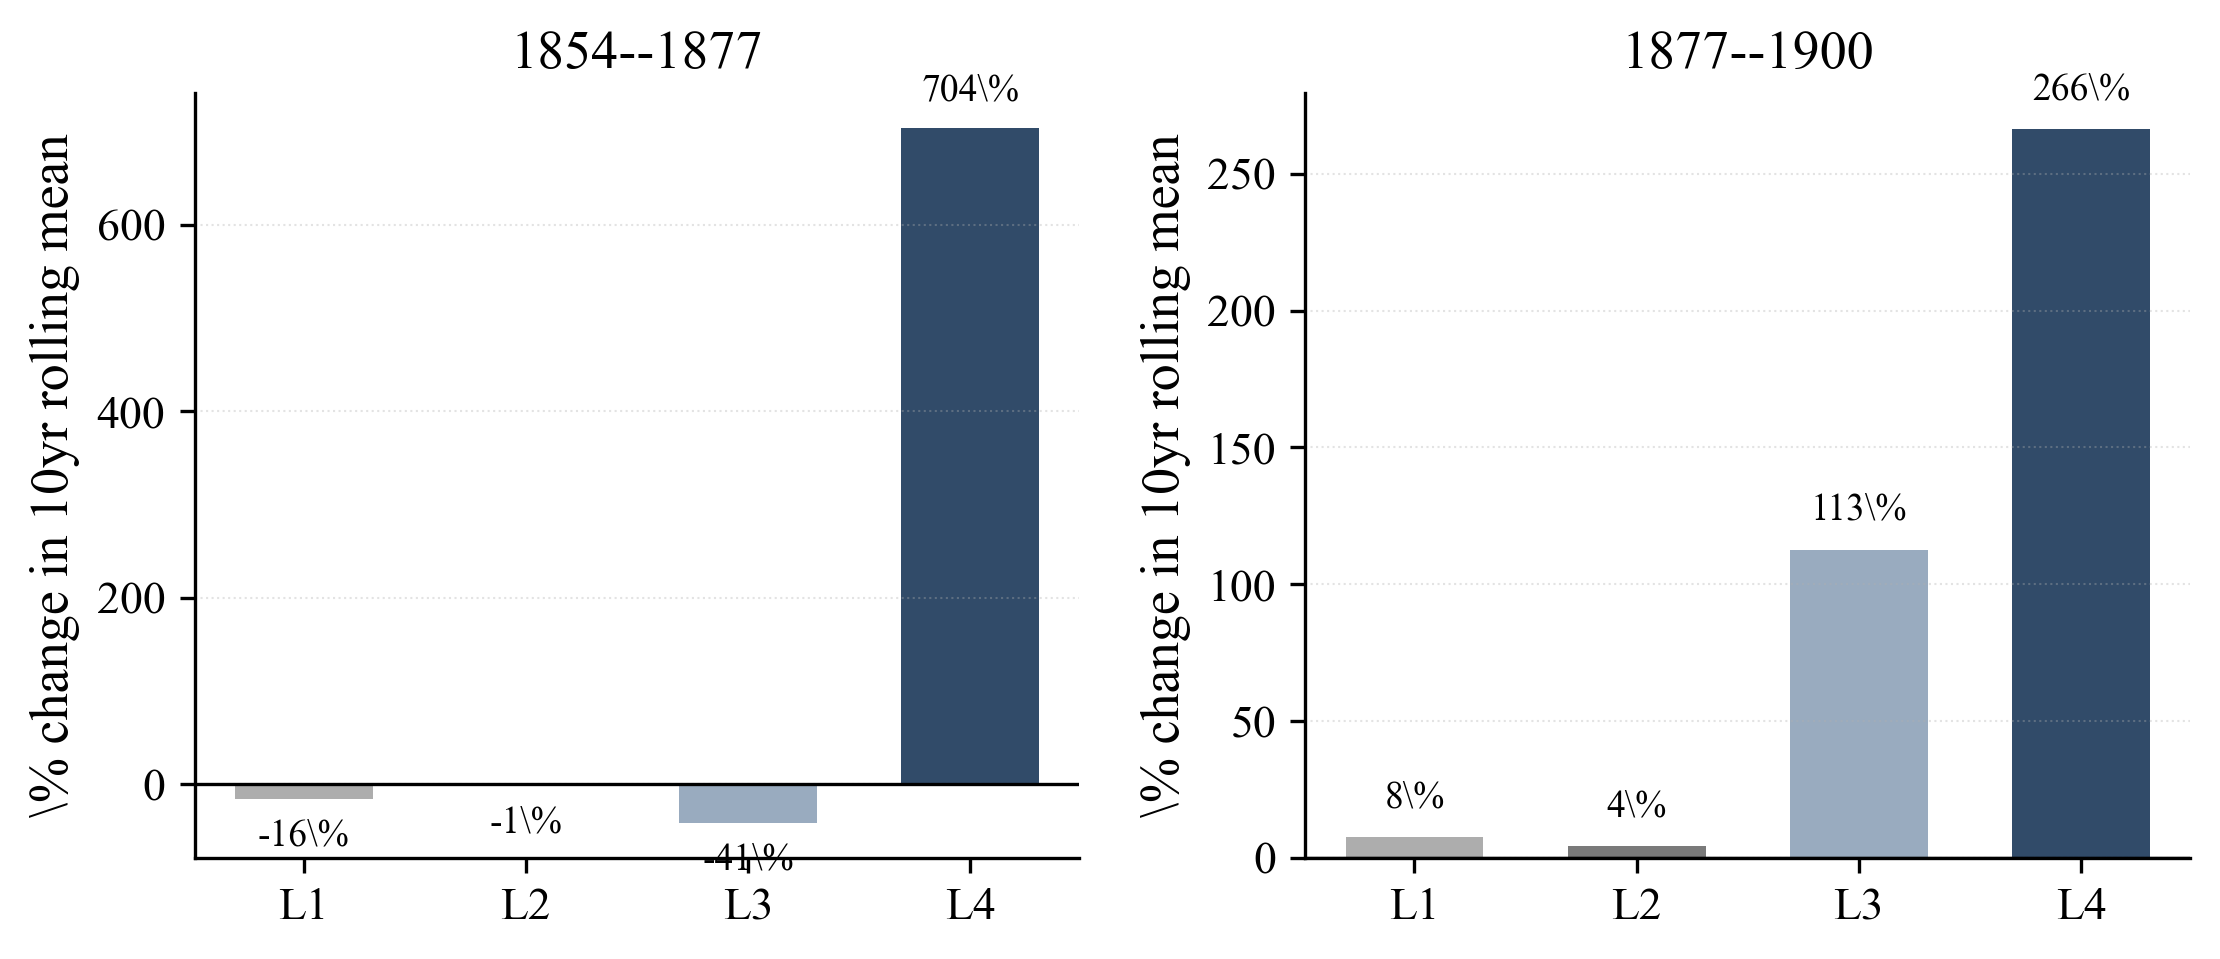
\includegraphics[width=0.80\textwidth]{figures/figA_acceleration.png}
\caption{Post-reform acceleration: \% change in 10-year rolling mean by depth and window.}
\label{fig:accel}
\end{figure}

\begin{figure}[H]
\centering
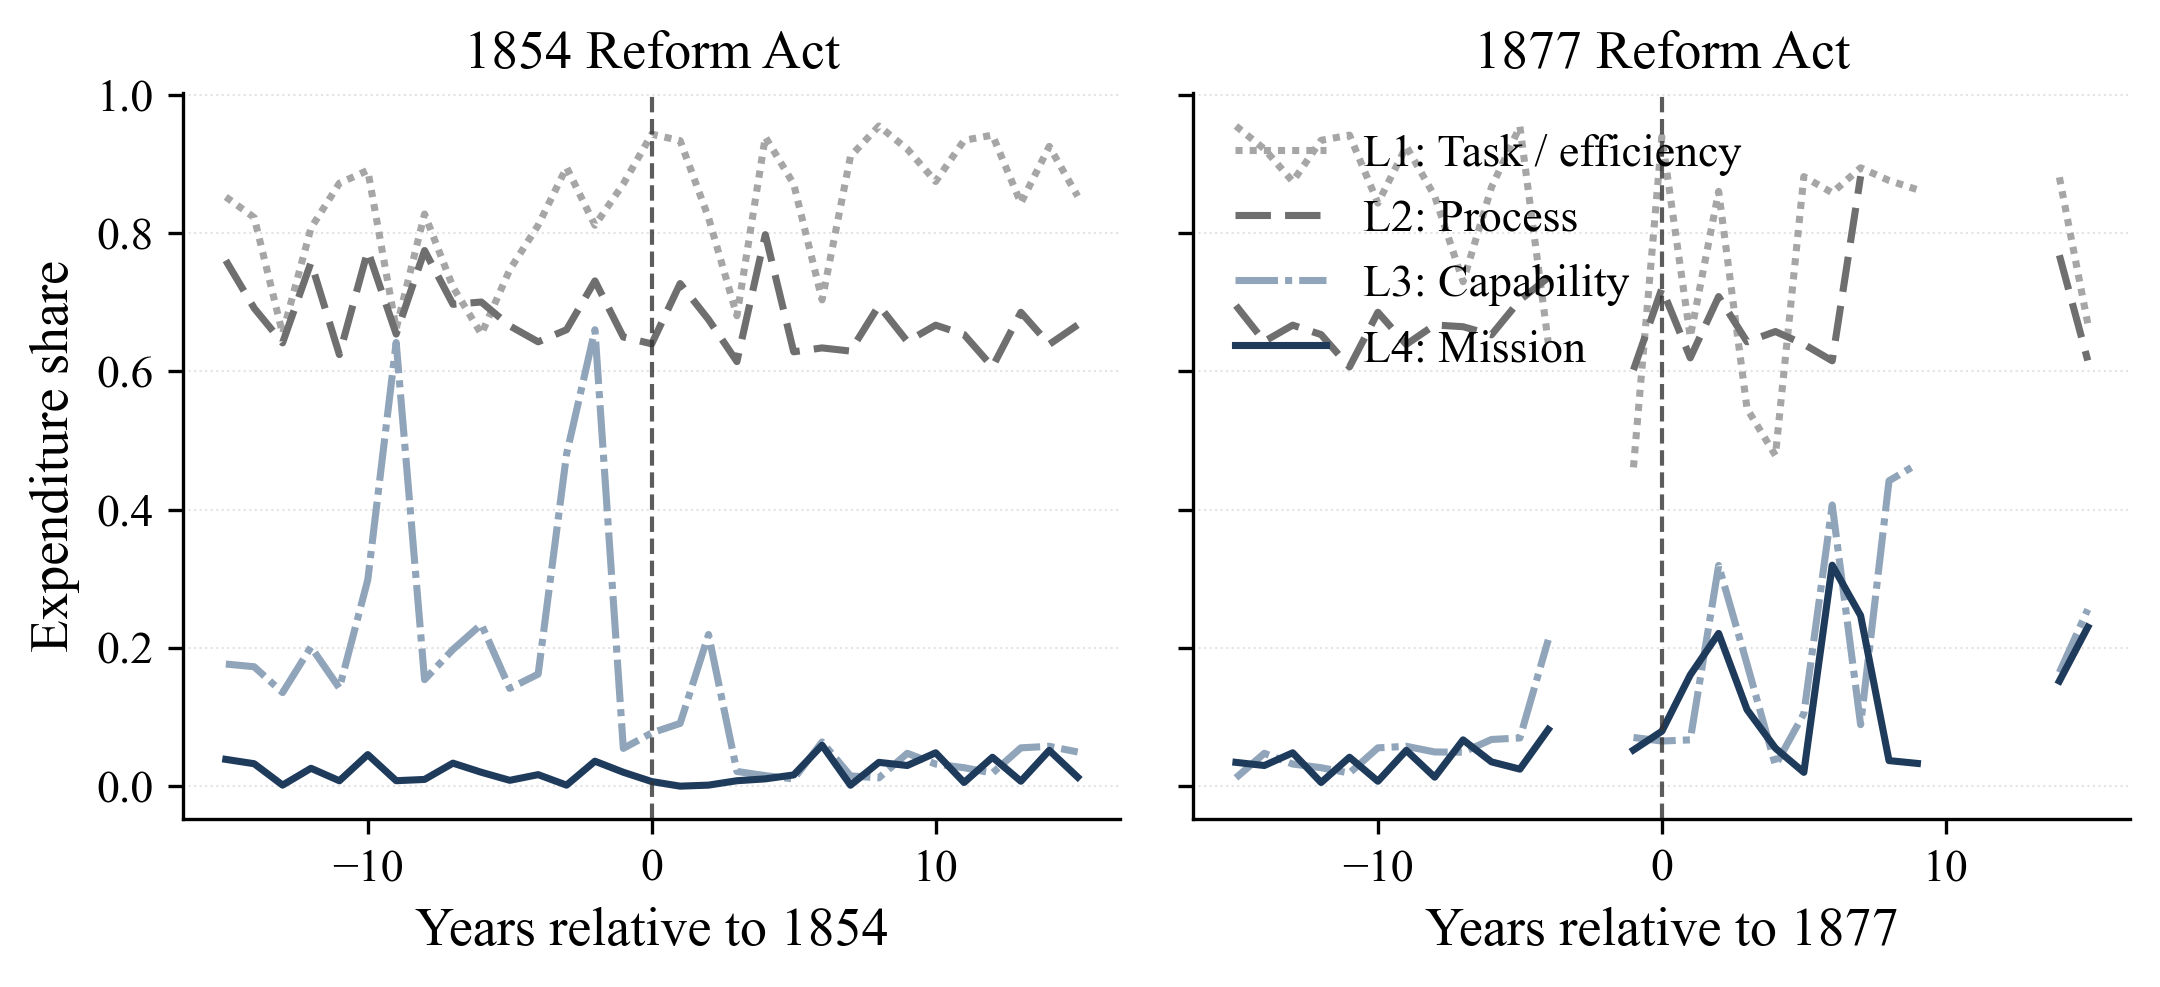
\includegraphics[width=0.80\textwidth]{figures/figA_eventtime.png}
\caption{Event-time response by depth in a $\pm 15$-year window around each Reform Act.}
\label{fig:event}
\end{figure}

% ===========================================================================
\section{Exploratory Results (Research Inventory)}
\label{app:inventory}
% ===========================================================================

Several patterns documented during the project are not central to the depth-asymmetry story and
are preserved here as candidate directions for future work, with their current evidentiary
status: (i)~capability-before-mission (L3-leads-L4) sequencing, direction consistent, but
cross-lag tests on first differences are not significant; (ii)~tests of strict
L1$\rightarrow$L2$\rightarrow$L3$\rightarrow$L4 ordering, partial change-point support, Granger
chaining mostly null; (iii)~the resource-slack lead-lag relationship between land-rent
income/financial capacity and the higher depths, co-moving but with confidence intervals that
include zero; (iv)~the Latin-to-English semantic transition in the corpus; (v)~income-source
diversification dynamics; and (vi)~the shift from personal to institutional payees. These are
maintained, with source artifacts, in the project research inventory.

\bibliographystyle{plainnat}
\bibliography{references}

\end{document}
